\section{Requisiti funzionali}
\label{secD2:RequisitiFunzionali}

Nel presente capitolo vengono riportati i requisiti funzionali del sistema utilizzando il linguaggio naturale e Use Case Diagram (UC) scritti in UML.

\begin{listaPersonale}[UC]{}
    \elemento[Use case “Accesso e registrazione” (\prettyref{D1-rf:AccessoRegistrazione})]{uc:AccessoRegistrazioneAccount}

    \begin{center}
        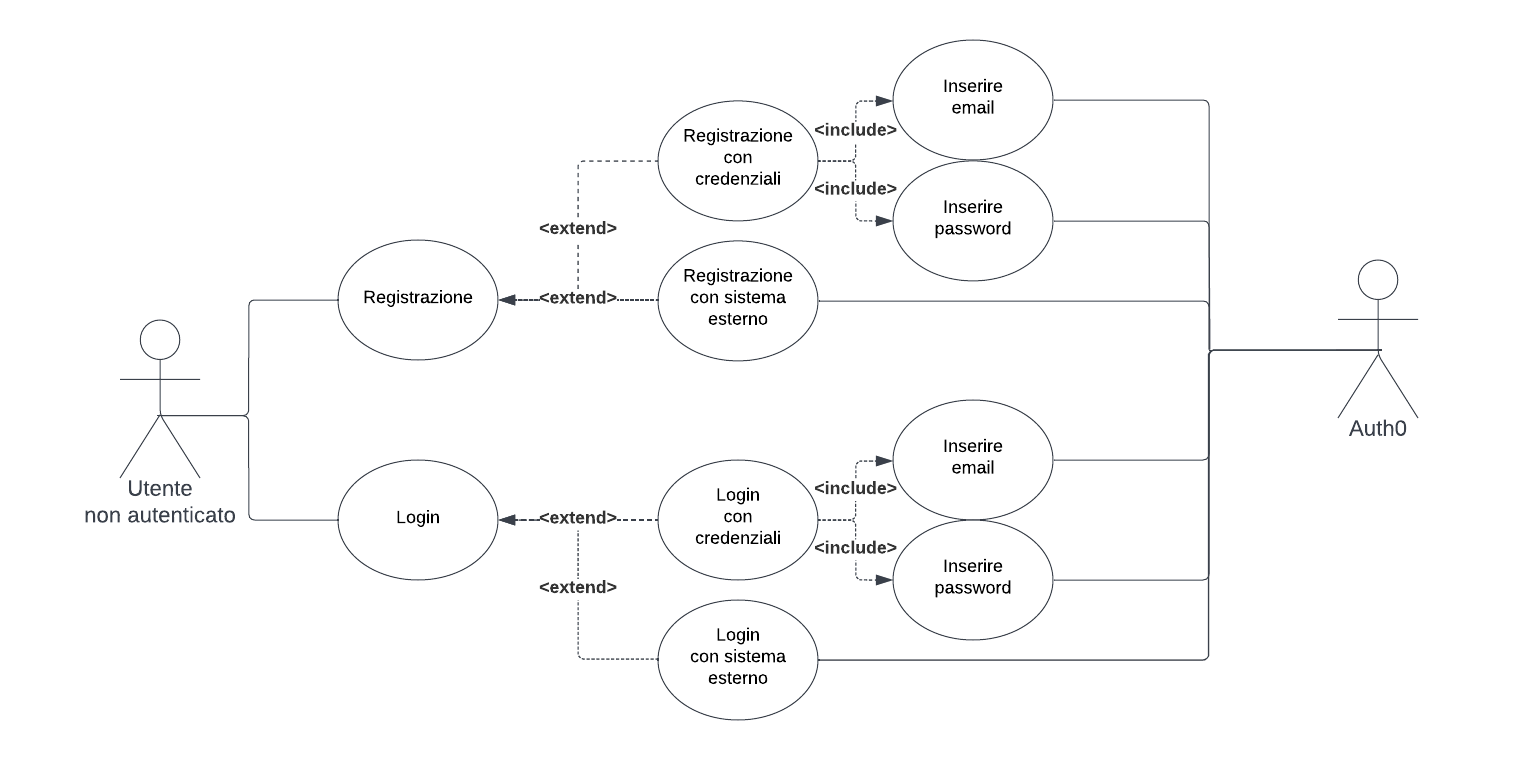
\includegraphics[width=0.7\textwidth]{img/Diagrammi/UseCases/AccessoRegistrazione.png}
    \end{center}
    In quanto le azioni di "Login" e "Registrazione" presentano molte procedure in comune, poichè c'è la partecipazione in comune di Auth0, che gestisce sia il login che la registrazione, abbiamo deciso di fare un State Machine Diagram con swimlanes che ingloba entrambi gli use case di "Login" e "Registrazione", anziché andare a fare due State Machine Diagram distinti, i quali avrebbero avuto molte ridondanze. \\ Lo State Machine Diagram prende in considerazione tutte le possibili procedure che l'utente non autenticato  può intraprendere a seconda delle sue scelte. Proprio queste scelte sono stato il motivo per cui abbiamo deciso di usare uno State Machine Diagram a discapito di una descrizione in italiano, in cui non è possibile andare a specificare la possibilità di scelta.

    \textbf{Diagramma:}
    \begin{center}
        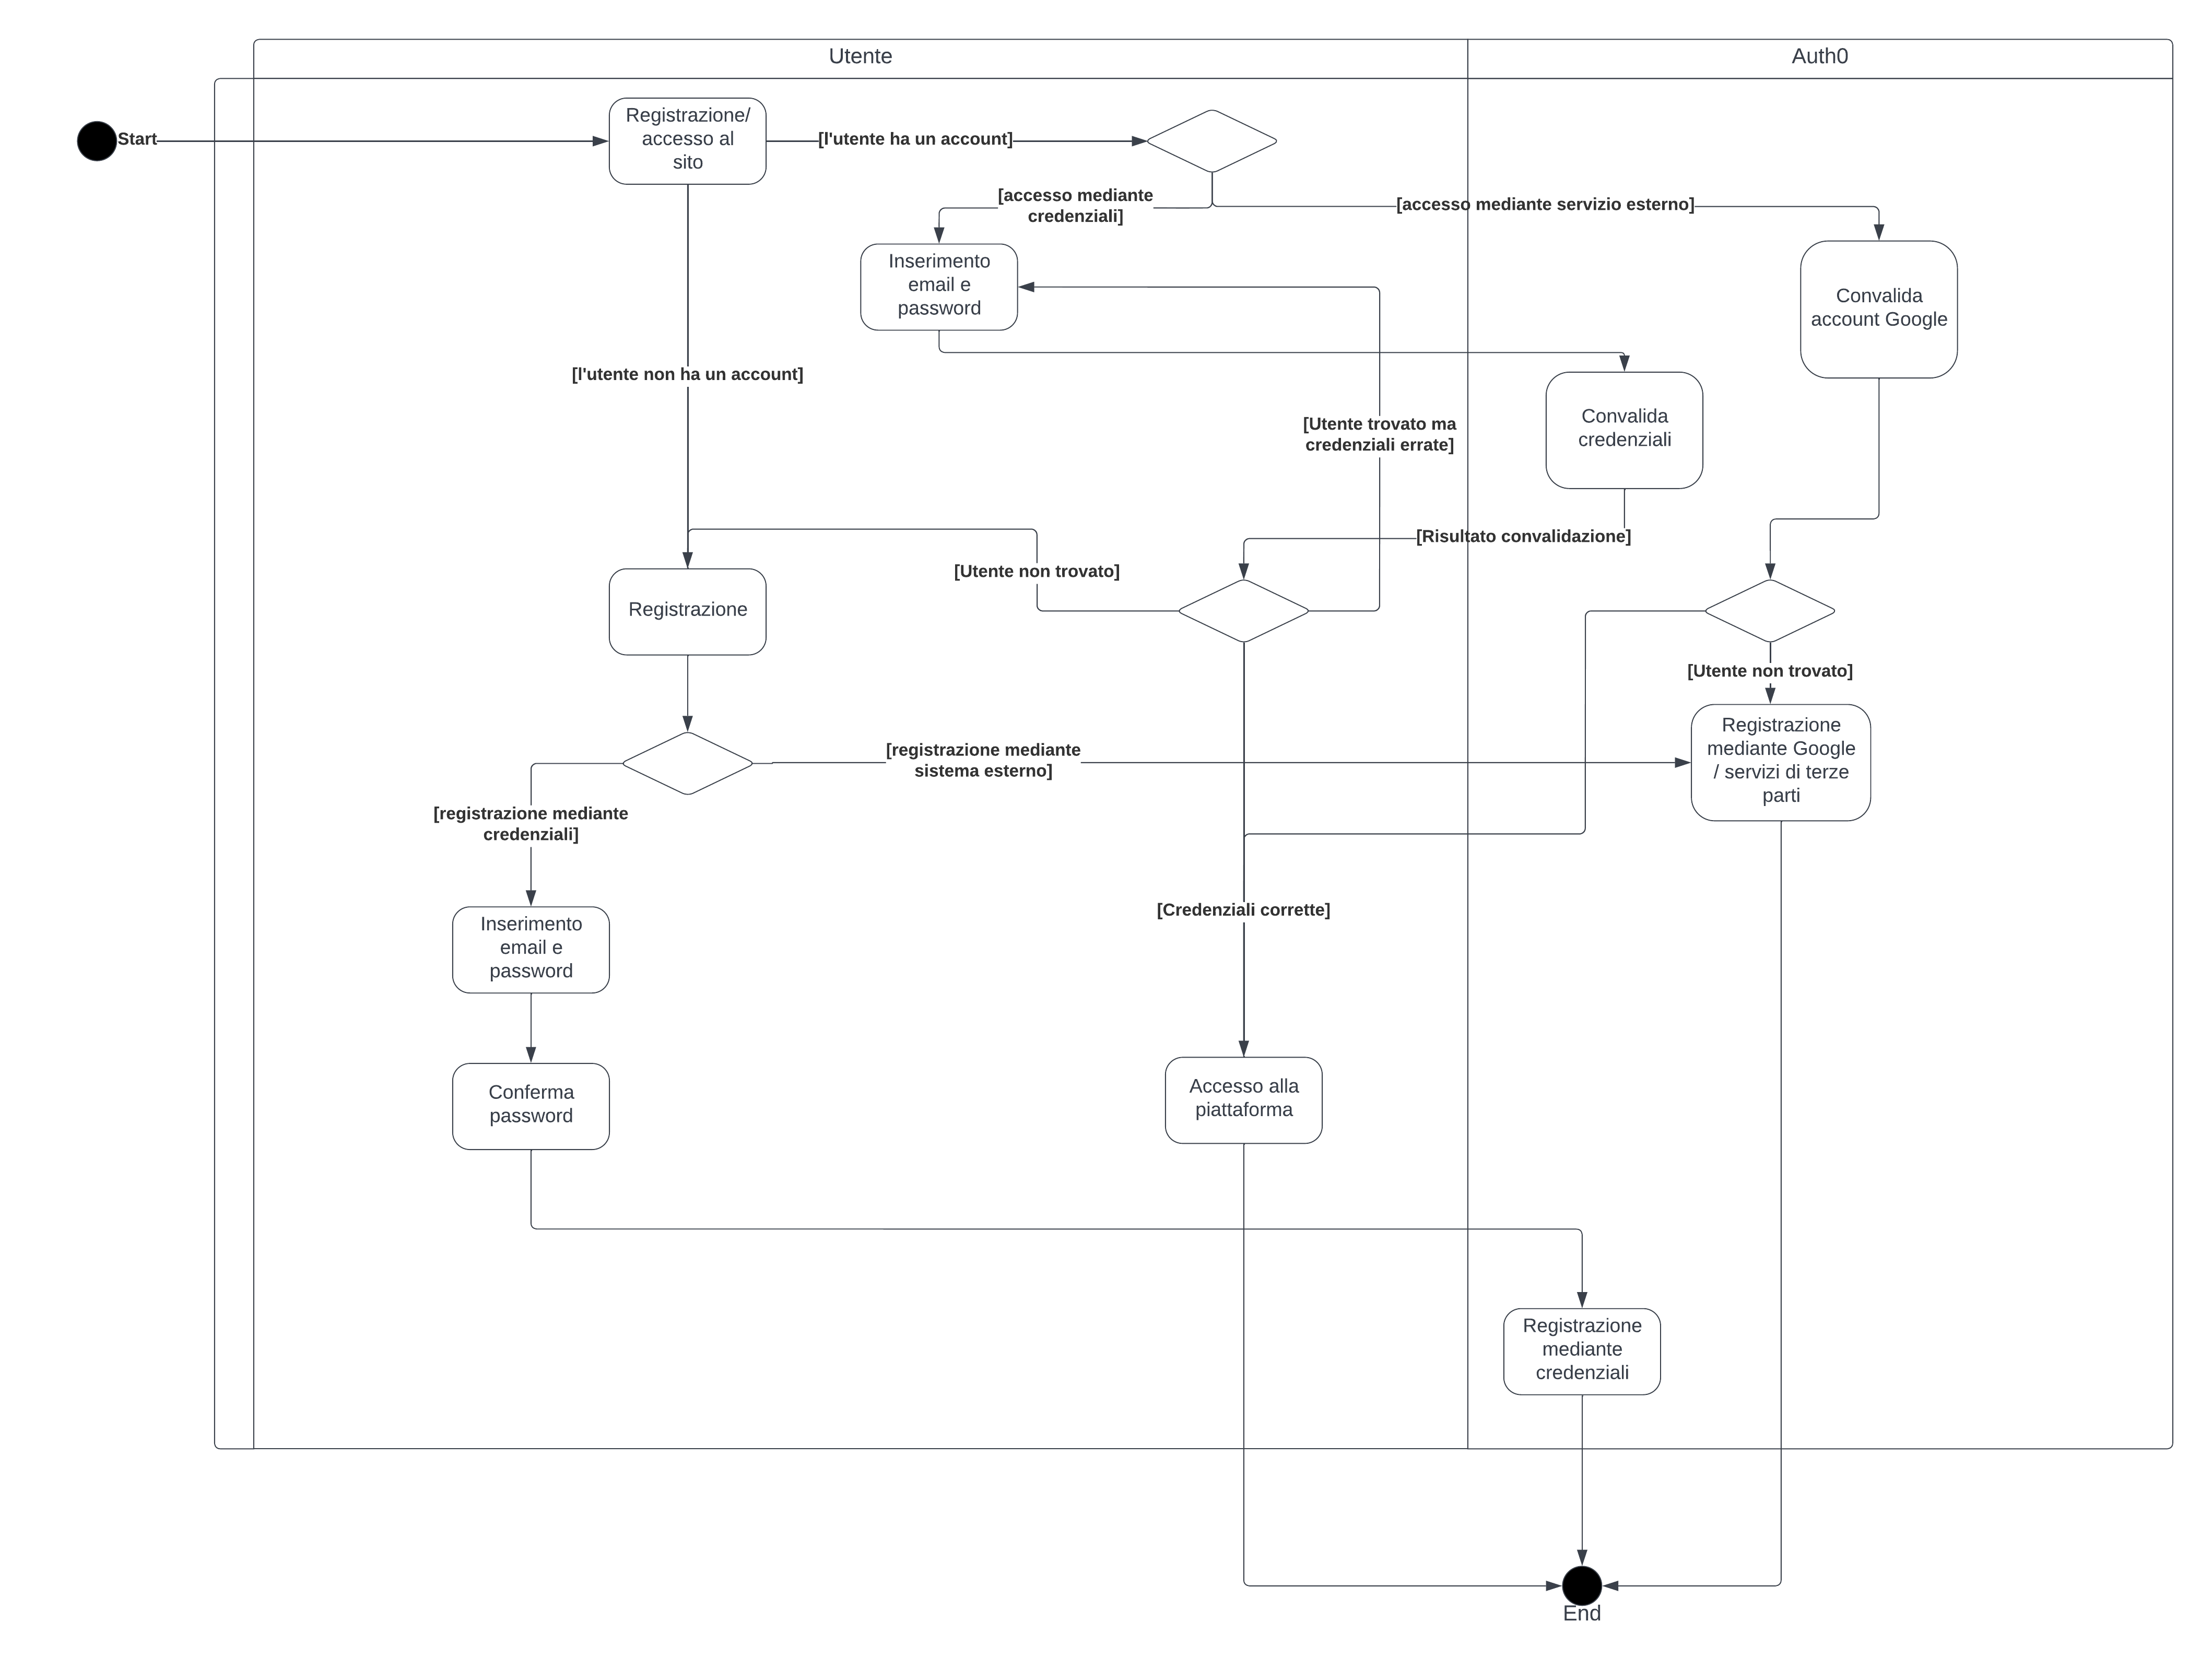
\includegraphics[width=1\textwidth, height = 0.4\textheight]{img/Diagrammi/DS/DS_AccessoRegistrazione.png}
    \end{center}


    \newpage
    \elemento[“Funzionalità di ciascuna tipologia di account” (\prettyref{D1-rf:UtenteNonAutenticato}, \prettyref{D1-rf:UtenteStandard}, \prettyref{D1-rf:UtentePremium})]{uc:TipiAccount}


    \begin{center}
        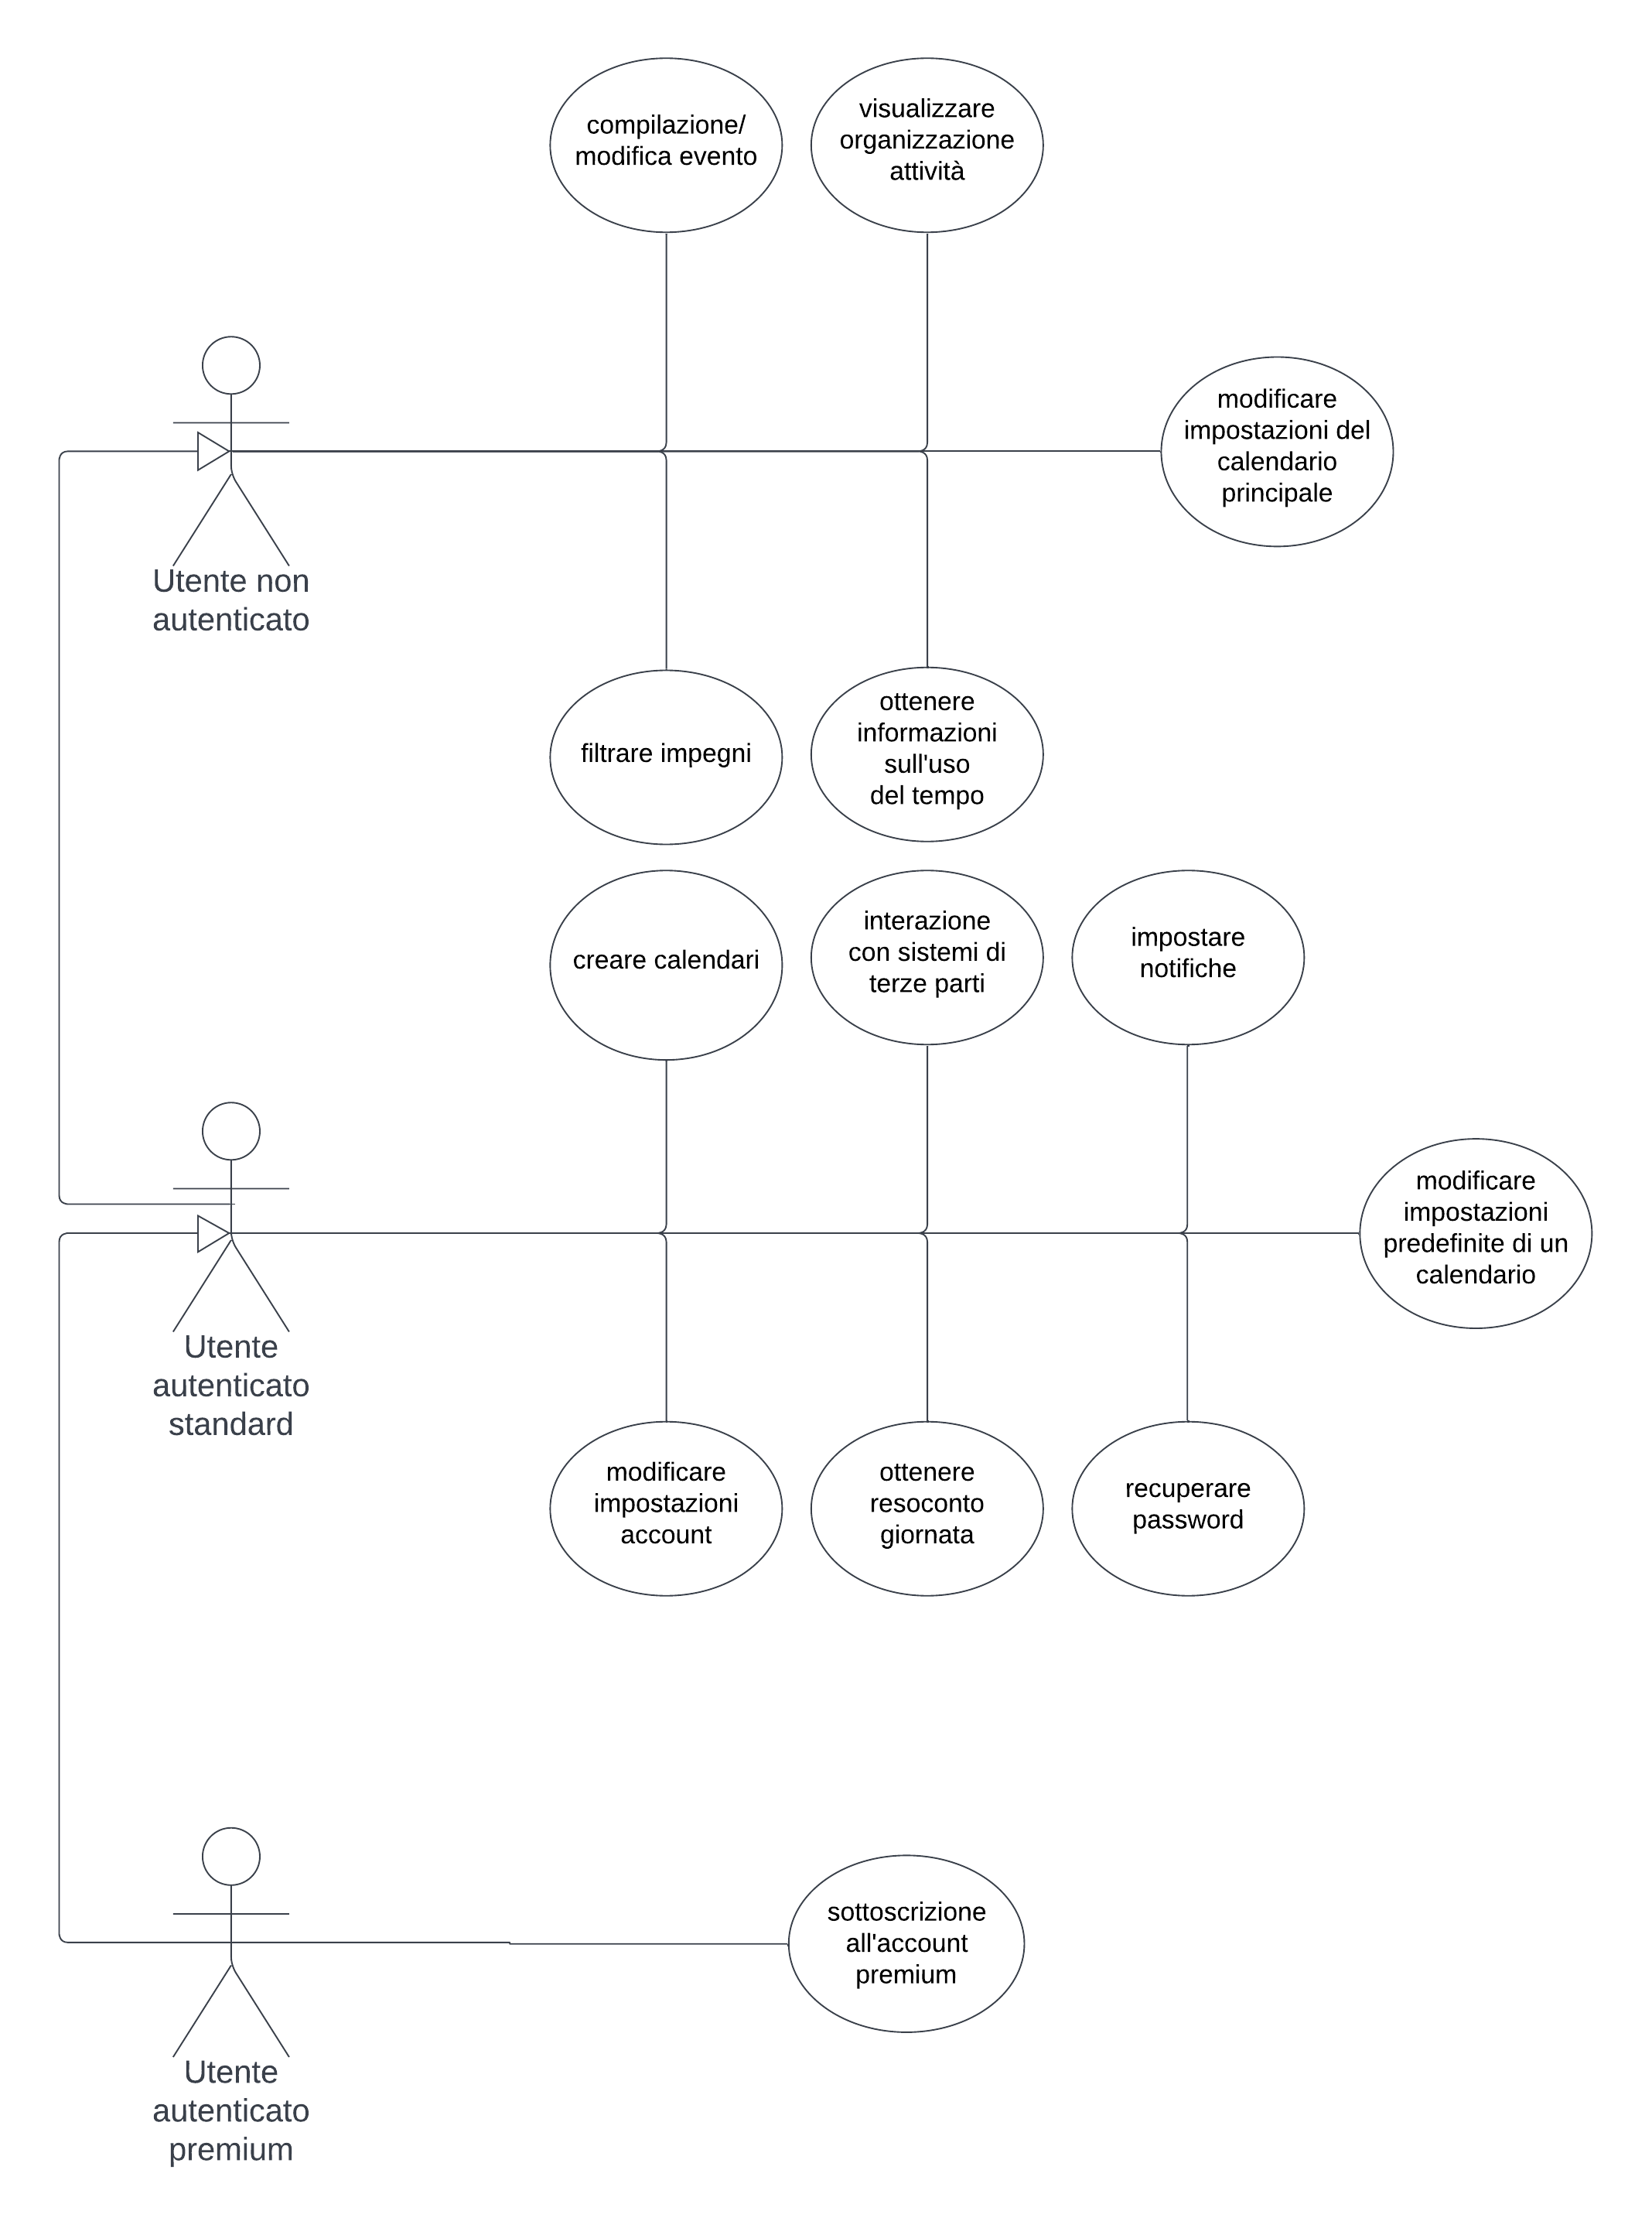
\includegraphics[width=0.6\textwidth, height = 0.5\textheight]{img/Diagrammi/UseCases/FunzionalitaUtenti.png}
    \end{center}
    \begin{listaPersonale2} [UC] {}
        \elemento [Titolo: Use case funzionalità utente non autenticato(\prettyref{D1-rf:UtenteNonAutenticato})] {uc:UtenteNonAutenticato}
        \textbf{Riassunto:} \\
        Questo use case presenta a livello generale quali sono le funzionalità presenti per l'utente non autenticato. Tutte le funzionalità, presentate nella descrizione, sono descritte dettagliatamente nei prossimi use case, che entreranno più nello specifico per ciascuna funzionalità.

        \textbf{Descrizione:}
        L'utente non autenticato, grazie alla modalità demo del sito, può accedere alle seguenti funzionalità:
        \begin{itemize}
            \item aggiunta e modifica di un evento;
            \item organizzare attività;
            \item modificare impostazioni del calendario principale;
            \item ottenere informazioni sull'uso del tempo;
            \item filtrare gli impegni.
        \end{itemize}

        \elemento [Titolo: Use case funzionalità utente autenticato standard (\prettyref{D1-rf:UtenteStandard})] {uc:UtenteAutenticatoStandard}
        \textbf{Riassunto:} \\
        Questo use case presenta a livello generale quali sono le funzionalità accessibili per l'utente autenticato standard. Tutte le funzionalità, presentate nella descrizione, sono descritte con maggiore dettaglio nei prossimi use case, che entreranno più nello specifico per ciascuna funzionalità. \\
        \textbf{Descrizione:}
        L'utente autenticato standard oltre alle funzionalità di un utente demo potrà accedere alle seguenti funzionalità:
        \begin{itemize}
            \item creare calendari;
            \item interazione con sistemi di terze parti;
            \item impostare notifiche;
            \item modificare impostazioni predefinite di un calendario oltre a quello principale;
            \item recuperare password;
            \item ottenere resoconto giornata;
            \item modificare le impostazioni dell'account.
        \end{itemize}
        \elemento[Titolo: Use case funzionalità utente autenticato premium (\prettyref{D1-rf:UtentePremium})] {uc:UtenteAutenticatoPremium} 
        \textbf{Riassunto:} \\
        Questo use case presenta a livello generale quali sono le funzionalità presenti per l'utente autenticato premium. Tutte le funzionalità, presentate nella descrizione, sono descritte con maggiore dettaglio nei prossimi use case, che entreranno più nello specifico per ciascuna funzionalità. \\
        \textbf{Descrizione:} \\
        L'utente autenticato premium, oltre alle funzionalità di un utente autenticato standard, può accedere anche alla seguente funzionalità:
        \begin{itemize}
            \item sottoscrizione all'account premium, mediante un pagamento mensile.
        \end{itemize}
    \end{listaPersonale2}
    Specifichiamo che tutti gli use case validi per l'utente non autenticato, lo sono anche per quello autenticato standard e premium. Allo stesso modo gli use case per l'utente autenticato standard sono validi anche per l'utente autenticato premium.
    \newpage

    \elemento[Use case “Gestione di calendari” (\prettyref{D1-rf:CondivisioneCalendario})]{uc:GestioneCalendari}


    \begin{center}
        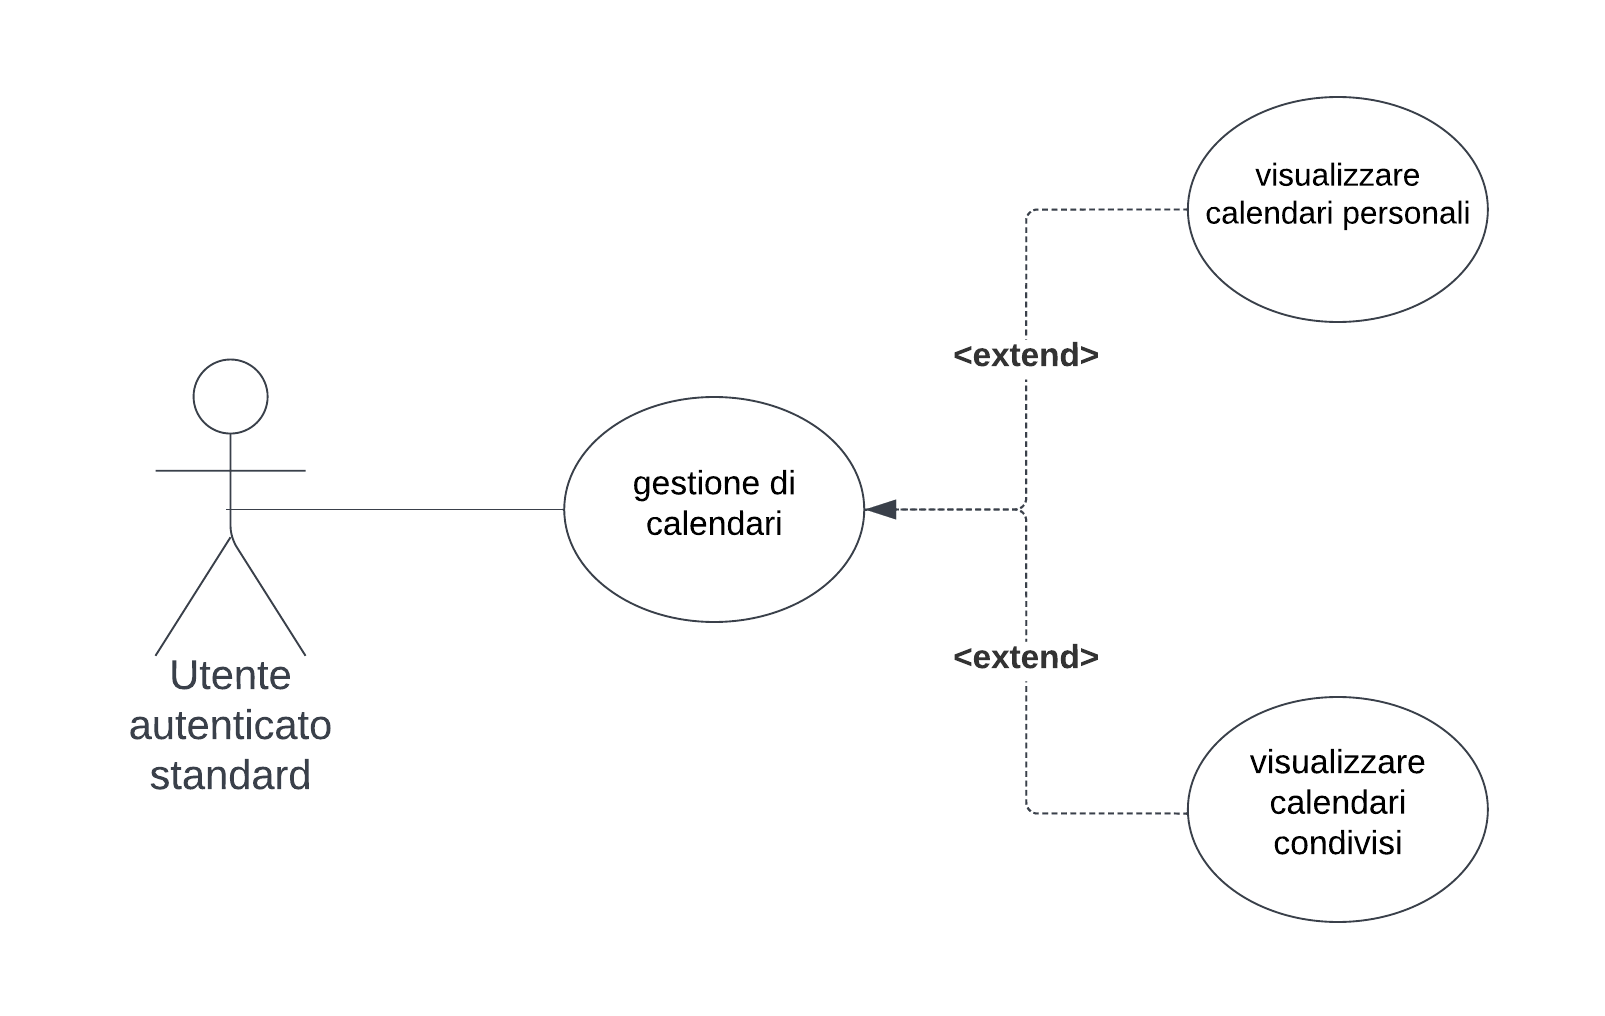
\includegraphics[width=0.7\textwidth]{img/Diagrammi/UseCases/CondivisioneCalendario.png}
    \end{center}

    \textbf{Titolo:} gestione di calendari

    \textbf{Riassunto:} \\
    Questo use descrive come l'utente autenticato standard può visualizzare e gestire i calendari personali e quelli condivisi.

    \textbf{Descrizione:}
    \begin{enumerate}
        \item Dalla sezione "Calendari", l'utente può visualizzare e gestire i suoi calendari personali e i calendari condivisi con altre persone.
        \item L'utente autenticato standard, da questa sezione, può selezionare quali calendari far apparire nella schermata “Calendario” in modo tale da osservare quali siano gli eventi presenti in un calendario specifico.
        \item Aprendo la sottosezione del calendario “Principale”, l'utente visualizza tutti i suoi calendari personali riguardo alle varie attività da svolgere. Il numero di calendari personali dipende dal tipo di account dell'utente autenticato: l'utente autenticato standard può avere al massimo cinque calendari personali, invece l'utente autenticato premium può averne un numero illimitato.
        \item Sotto il calendario “Principale”, sono presenti tutti i calendari condivisi (\ref{uc:ExtensionVisualizzazioneCalendariCondivisi}). Il numero di calendari condivisi che può avere un utente autenticato dipende dalla tipologia di account: l'utente autenticato standard può avere al massimo tre calendari condivisi, invece l'utente autenticato premium può averne un numero illimitato.
    \end{enumerate}


    \textbf{Extension:}
    \begin{enumerate}[label=\textbf{[extension \arabic{enumii}]}, ref= \textbf{[extension \arabic{enumii}]}]
        \elemento{uc:ExtensionVisualizzazioneCalendariCondivisi} L'utente autenticato standard può visualizzare quali siano i calendari condivisi anche osservando una piccola immagine stilizzata di persone alla destra del nome dei calendari condivisi (\prettyref{D1-fe:SchermataPrincipaleCalendario})
    \end{enumerate}




    \newpage
    \elemento[Use case “Creazione/modifica evento” (\prettyref{D1-rf:CreazioneModificaEvento})]{uc:CreazioneModificaEvento}

    \begin{center}
        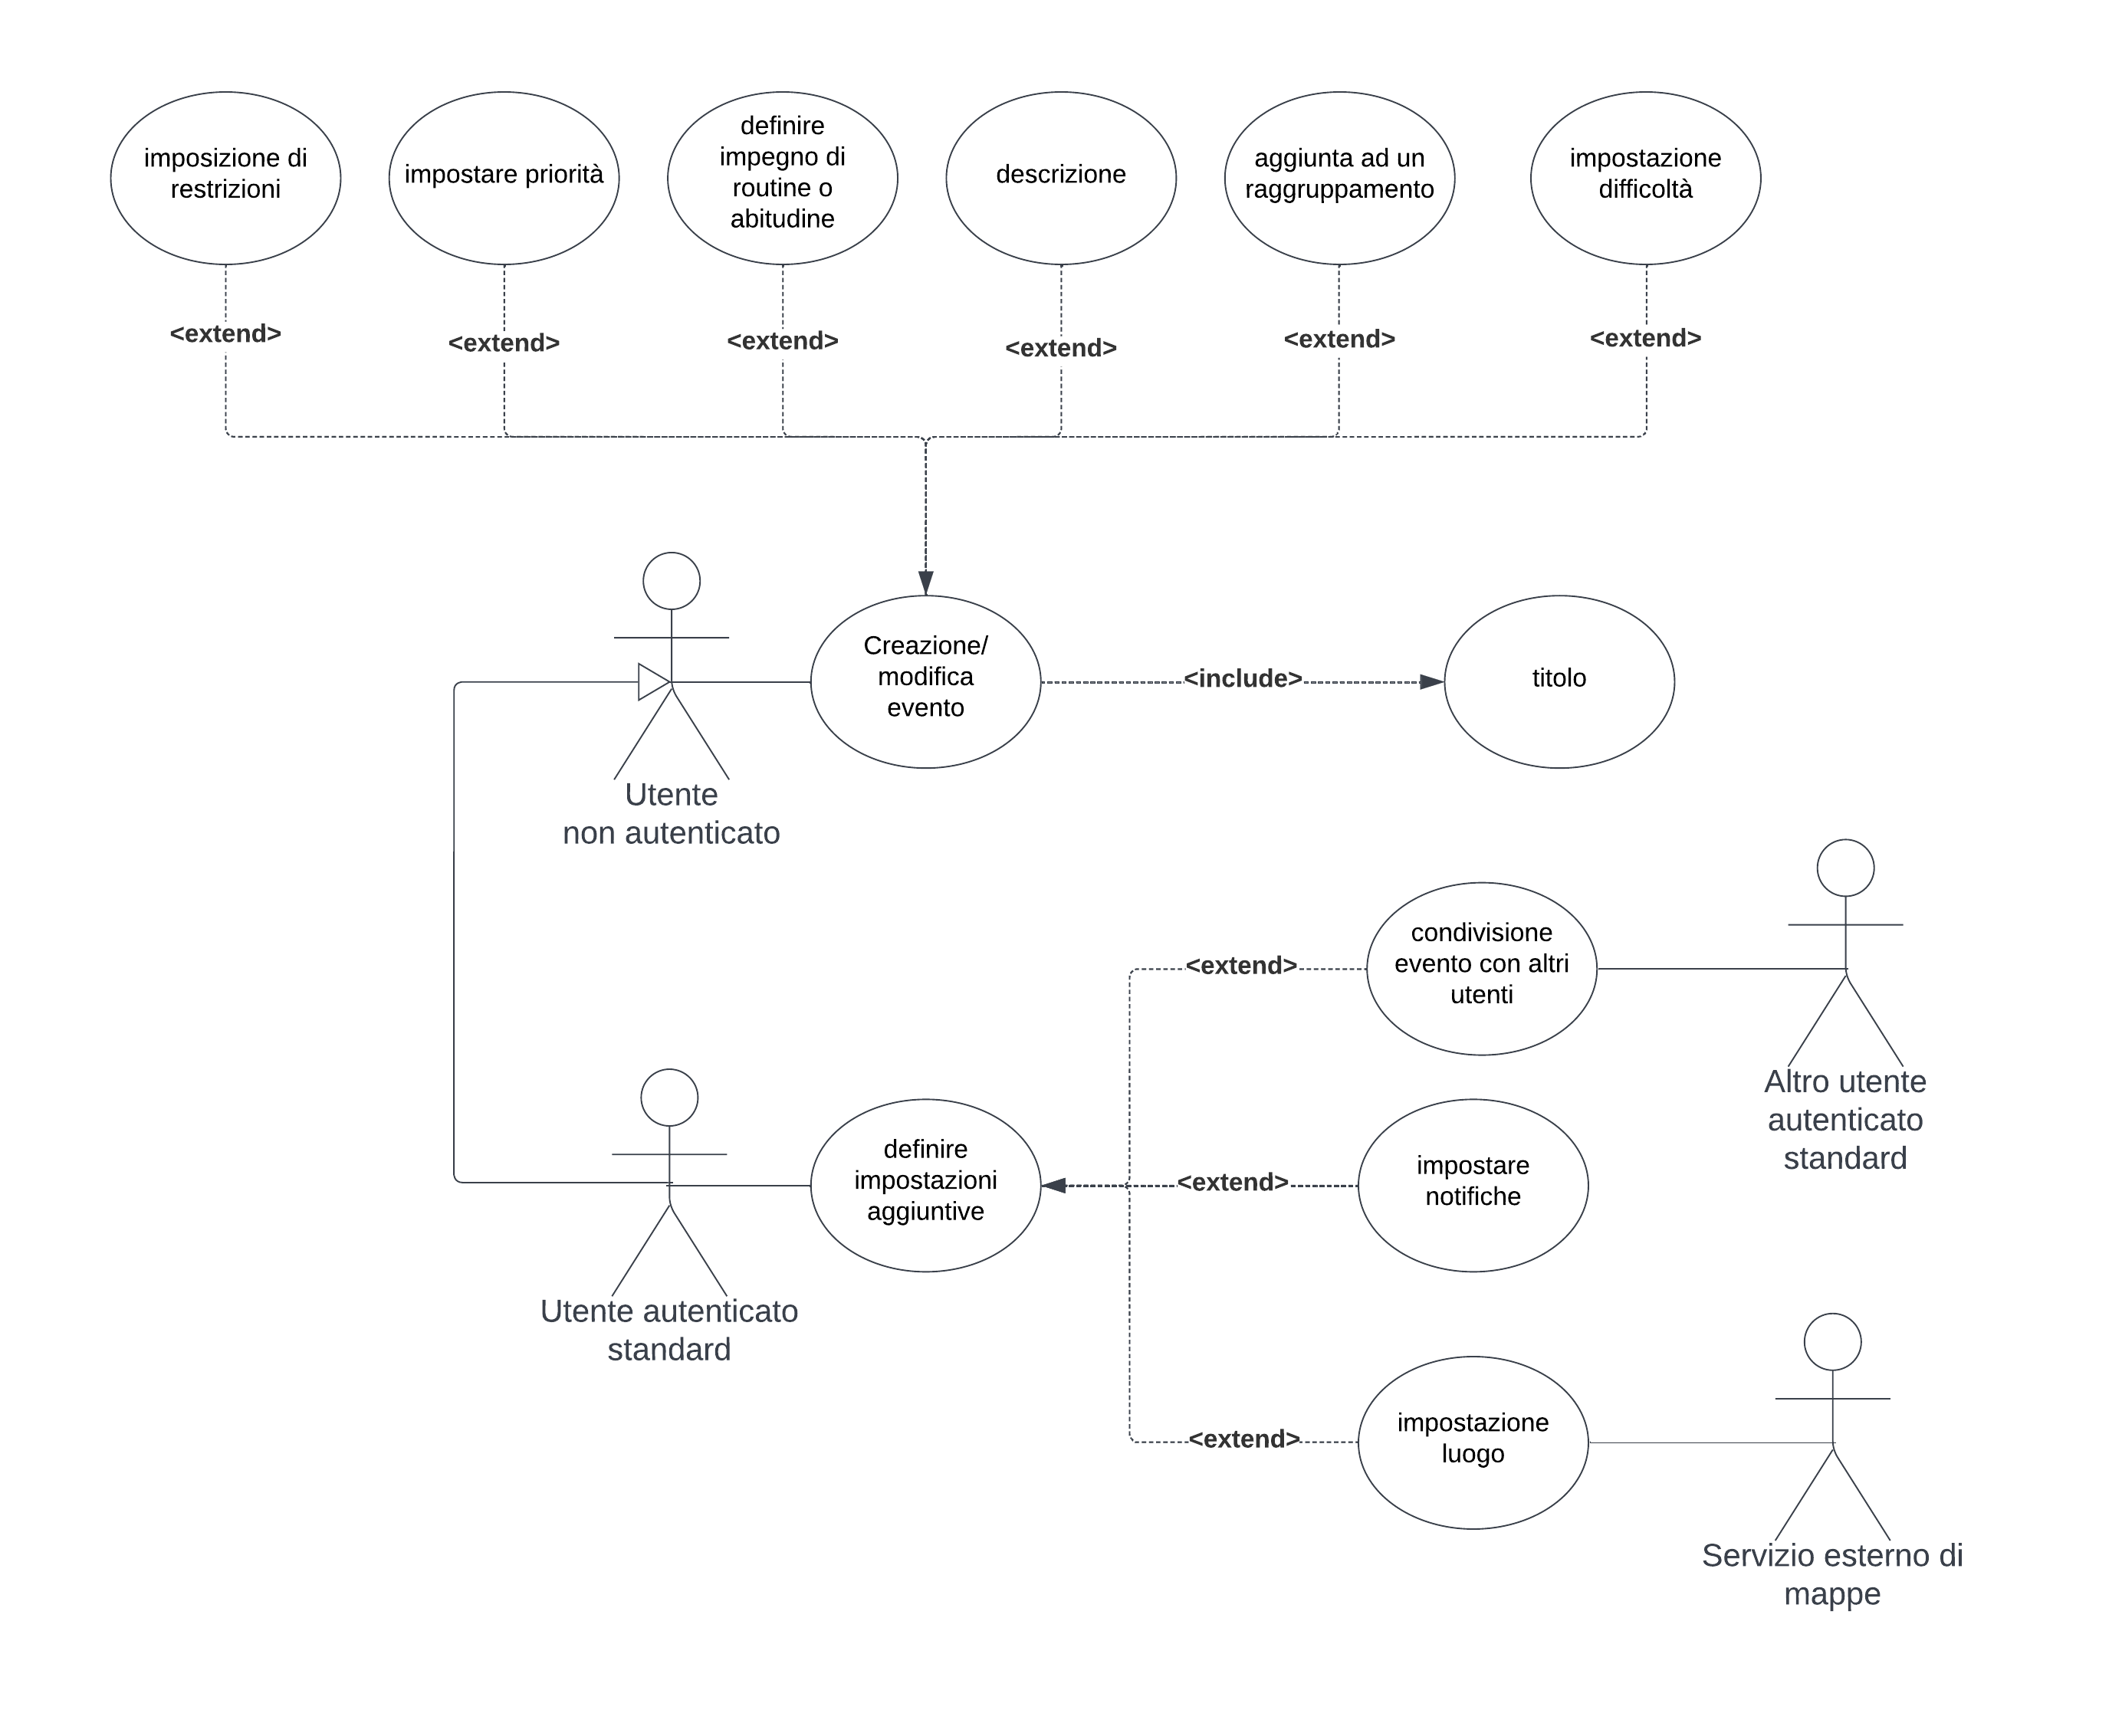
\includegraphics[width=0.85\textwidth, height = 0.5\textheight]{img/Diagrammi/UseCases/CreazioneModificaEvento.png}
    \end{center}
    Per andare a descrivere questo use case si è deciso di utilizzare un Activity Diagram con swimlanes, in quanto, in questo use case, sono presenti delle fork, join e anche delle scelte che possono essere effettuate da parte dell'utente non autenticato o autenticato standard. Inoltre, non si è diviso l'Activate Diagram in due parti, a seconda della tipologia di account, in quanto se ci fossero due diagrammi, questi avrebbero molto ridondanze. Infatti, come si può notare dall'Use Case Diagram, l'utente autenticato standard presenta le stesse funzionalità di quello non autenticato, avendo anche delle funzionalità aggiuntive.
    \newpage

    \textbf{Diagramma:}
    \begin{center}
        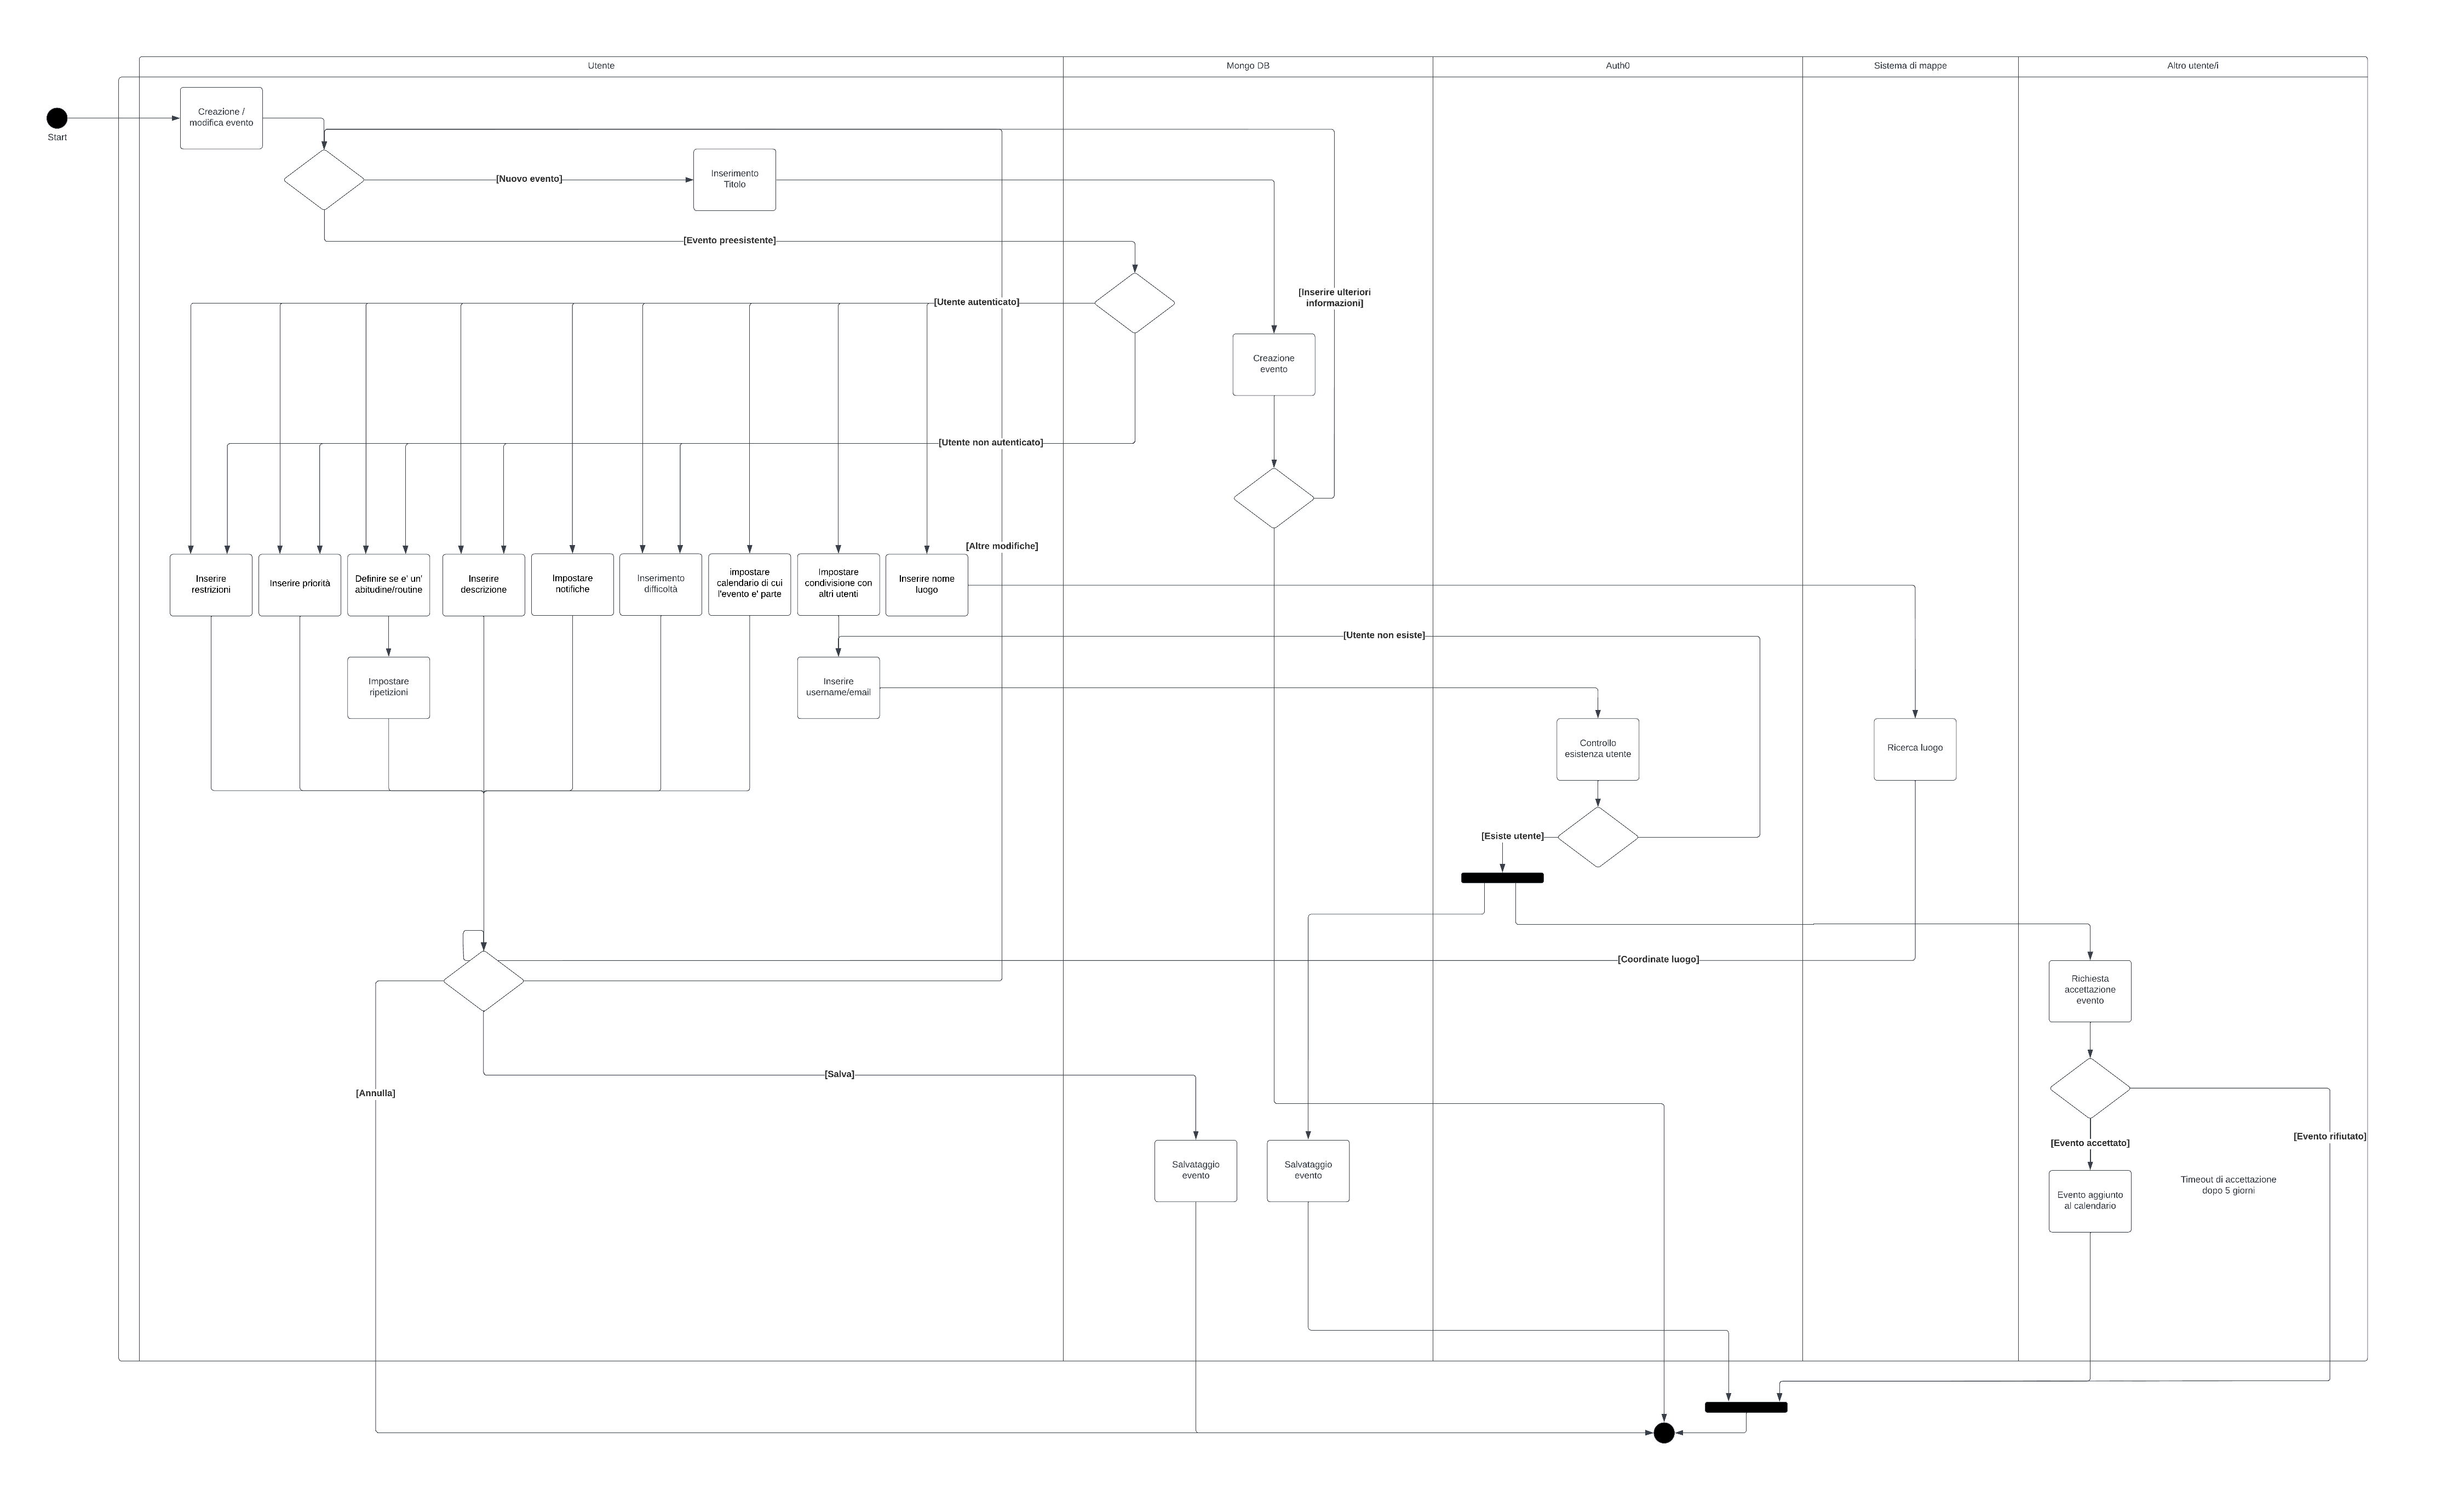
\includegraphics[width=1.1\textwidth, height = 0.4\textheight]{img/Diagrammi/DS/DS_CreazioneModificaEvento.png}
        Si prega di zoomare a piacere in modo tale di poter leggere bene le varie parti del diagramma
    \end{center}




    \newpage
    \elemento[“Organizzazione attività” (\prettyref{D1-rf:InserimentoAutomaticoCalendario})]{uc:VisualizzazioneEventiCalendario}


    \begin{center}
        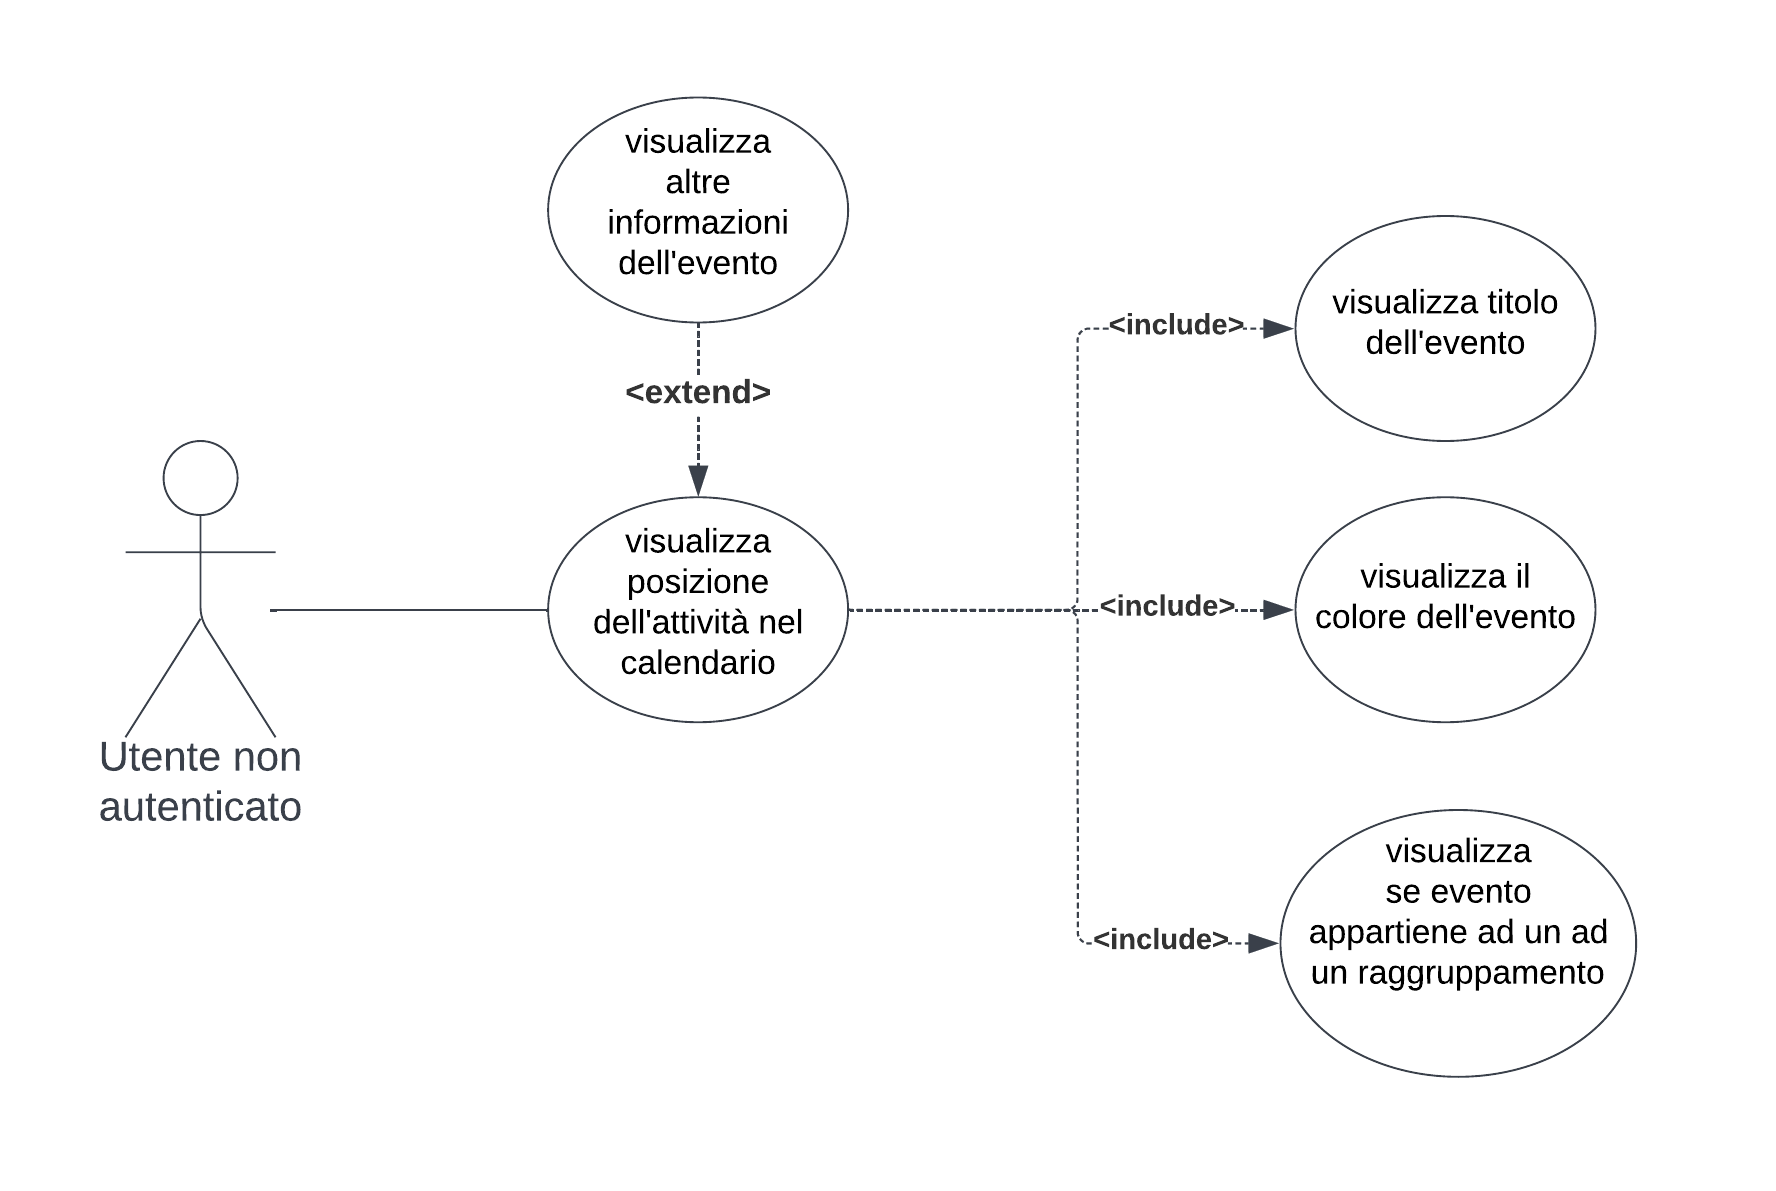
\includegraphics[width=0.7\textwidth]{img/Diagrammi/UseCases/InserimentoAutomaticoCalendario.png}
    \end{center}

    \begin{listaPersonale2} [UC] {}
    \elemento[Use case "Visualizza posizione dell'attività nel calendario"]{uc:VisualizzaEventiNonAutenticato}
    \textbf{Titolo:} Visualizzazione posizione dell'attività nel calendario \\
    \textbf{Riassunto: } \\
    Questo use case descrive come l'utente non autenticato visualizza l'evento nel proprio calendario e quali informazioni può ottenere dal blocco dell'evento presente nella schermata “Calendario”.

    \textbf{Descrizione: }
    \begin{enumerate}
        \item Dopo la compilazione dell'evento da aggiungere, l'utente non autenticato visualizza tale evento in un blocco nella schermata Calendario.
        \item Nel caso in cui l'utente non autenticato, in fase di compilazione dell'evento da aggiungere, non avesse definito data, ora e durata di tale attività, il sistema inserisce autonomamente e automaticamente l'impegno nel calendario secondo i seguenti criteri, i quali l'utente non autenticato può aver definito nella compilazione dell'evento (\ref{uc:ExceptionCampiNonCompilati}):
              \begin{itemize}
                  \item difficoltà dell' evento, ovvero quanto è complesso l'evento per completarlo;
                  \item priorità;
                  \item durata;
              \end{itemize}
        \item Dal blocco dell'evento nel calendario, l'utente non autenticato può visualizzare immediatamente alcune informazioni riguardo l'evento:
              \begin{itemize}
                  \item titolo;
                  \item colore dell'evento: da questa informazione l'utente non autenticato può comprendere a quale calendario appartiene l'evento; infatti il colore del blocco dell'evento corrisponde al colore del calendario a cui appartiene l'evento (ricordiamo che nel caso di utente non autenticato l'unico colore presente sarà quello del calendario “principale”, in quanto non avrà possibilità di creare altri calendari”).
              \end{itemize}
              \begin{comment} "può comprendere a quale calendario o raggruppamento appartiene l'evento" \end{comment}
        \item L'utente non autenticato premendo sull'evento fa apparire un pop-up dove può visualizzare tutte le informazioni di tale evento, ovvero tutte quelle sopra descritte e:
              \begin{itemize}
                  \item descrizione dell'evento;
                  \item se l'evento è un'abitudine;
                  \item difficoltà dell'evento;
                  \item nome del calendario di appartenenza
              \end{itemize}
        \item L'utente non autenticato, dopo aver visualizzato il pop-up in cui sono presenti tutte le informazioni riguardo l'evento, può tornare alla schermata precedente, ovvero "Calendario", premendo il tasto "Indietro".
        \end{enumerate}
        \elemento[Use case "Visualizza altre informazioni dell'evento"]{uc:VisualizzaEventoAutenticato}
        \textbf{Titolo: } Visualizzazione altre informazione dell'evento. \\
        \textbf{Riassunto: } \\ Questo use case descrive la possibilità data all'utente autenticato standard di visualizzare ulteriori informazioni riguardo l'evento, una volta che questo viene premuto.
        \textbf{Descrizione: }
        \begin{enumerate}
        \item Come si può notare dalla "generalizzazione" nell'use case, l'utente autenticato standard eredita dall'utente non autenticato tutte le sue funzionalità. Inoltre, nel pop-up di visualizzazione delle informazioni di un evento, l'utente autenticato standard visualizza ulteriori informazioni. 
        \item Nel caso di un utente autenticato standard, nel pop-up di visualizzazione di informazioni aggiuntive di un evento saranno presenti ulteriori campi, ovvero:
              \begin{itemize}
                  \item luogo dove si terrà l'evento; sarà presente la mappa con la segnalazione del luogo e anche il suo indirizzo;
                  \item lista di utenti a cui è condiviso l'evento;
                  \item quando è impostata la notifica dell'evento.
              \end{itemize}
    \end{enumerate}

    \textbf{Exceptions:}
    \begin{enumerate}[label=\textbf{[exception \arabic{enumiii}]}, ref= \textbf{[exception \arabic{enumiii}]}]
        \elemento{uc:ExceptionCampiNonCompilati} Nel caso in cui l'utente non autenticato non avesse definito questi campi in fase di creazione evento, sono presi i seguenti valori standard:
        \begin{itemize}
            \item priorità = 5;
            \item difficoltà = 5;
            \item durata = 1 ora;
        \end{itemize}
    \end{enumerate}
    \end{listaPersonale2}





    \newpage
    \elemento[Use case “Resoconto giornata” (\prettyref{D1-rf:ResocontoGiornata})]{uc:ResocontoGiornata}


    \begin{center}
        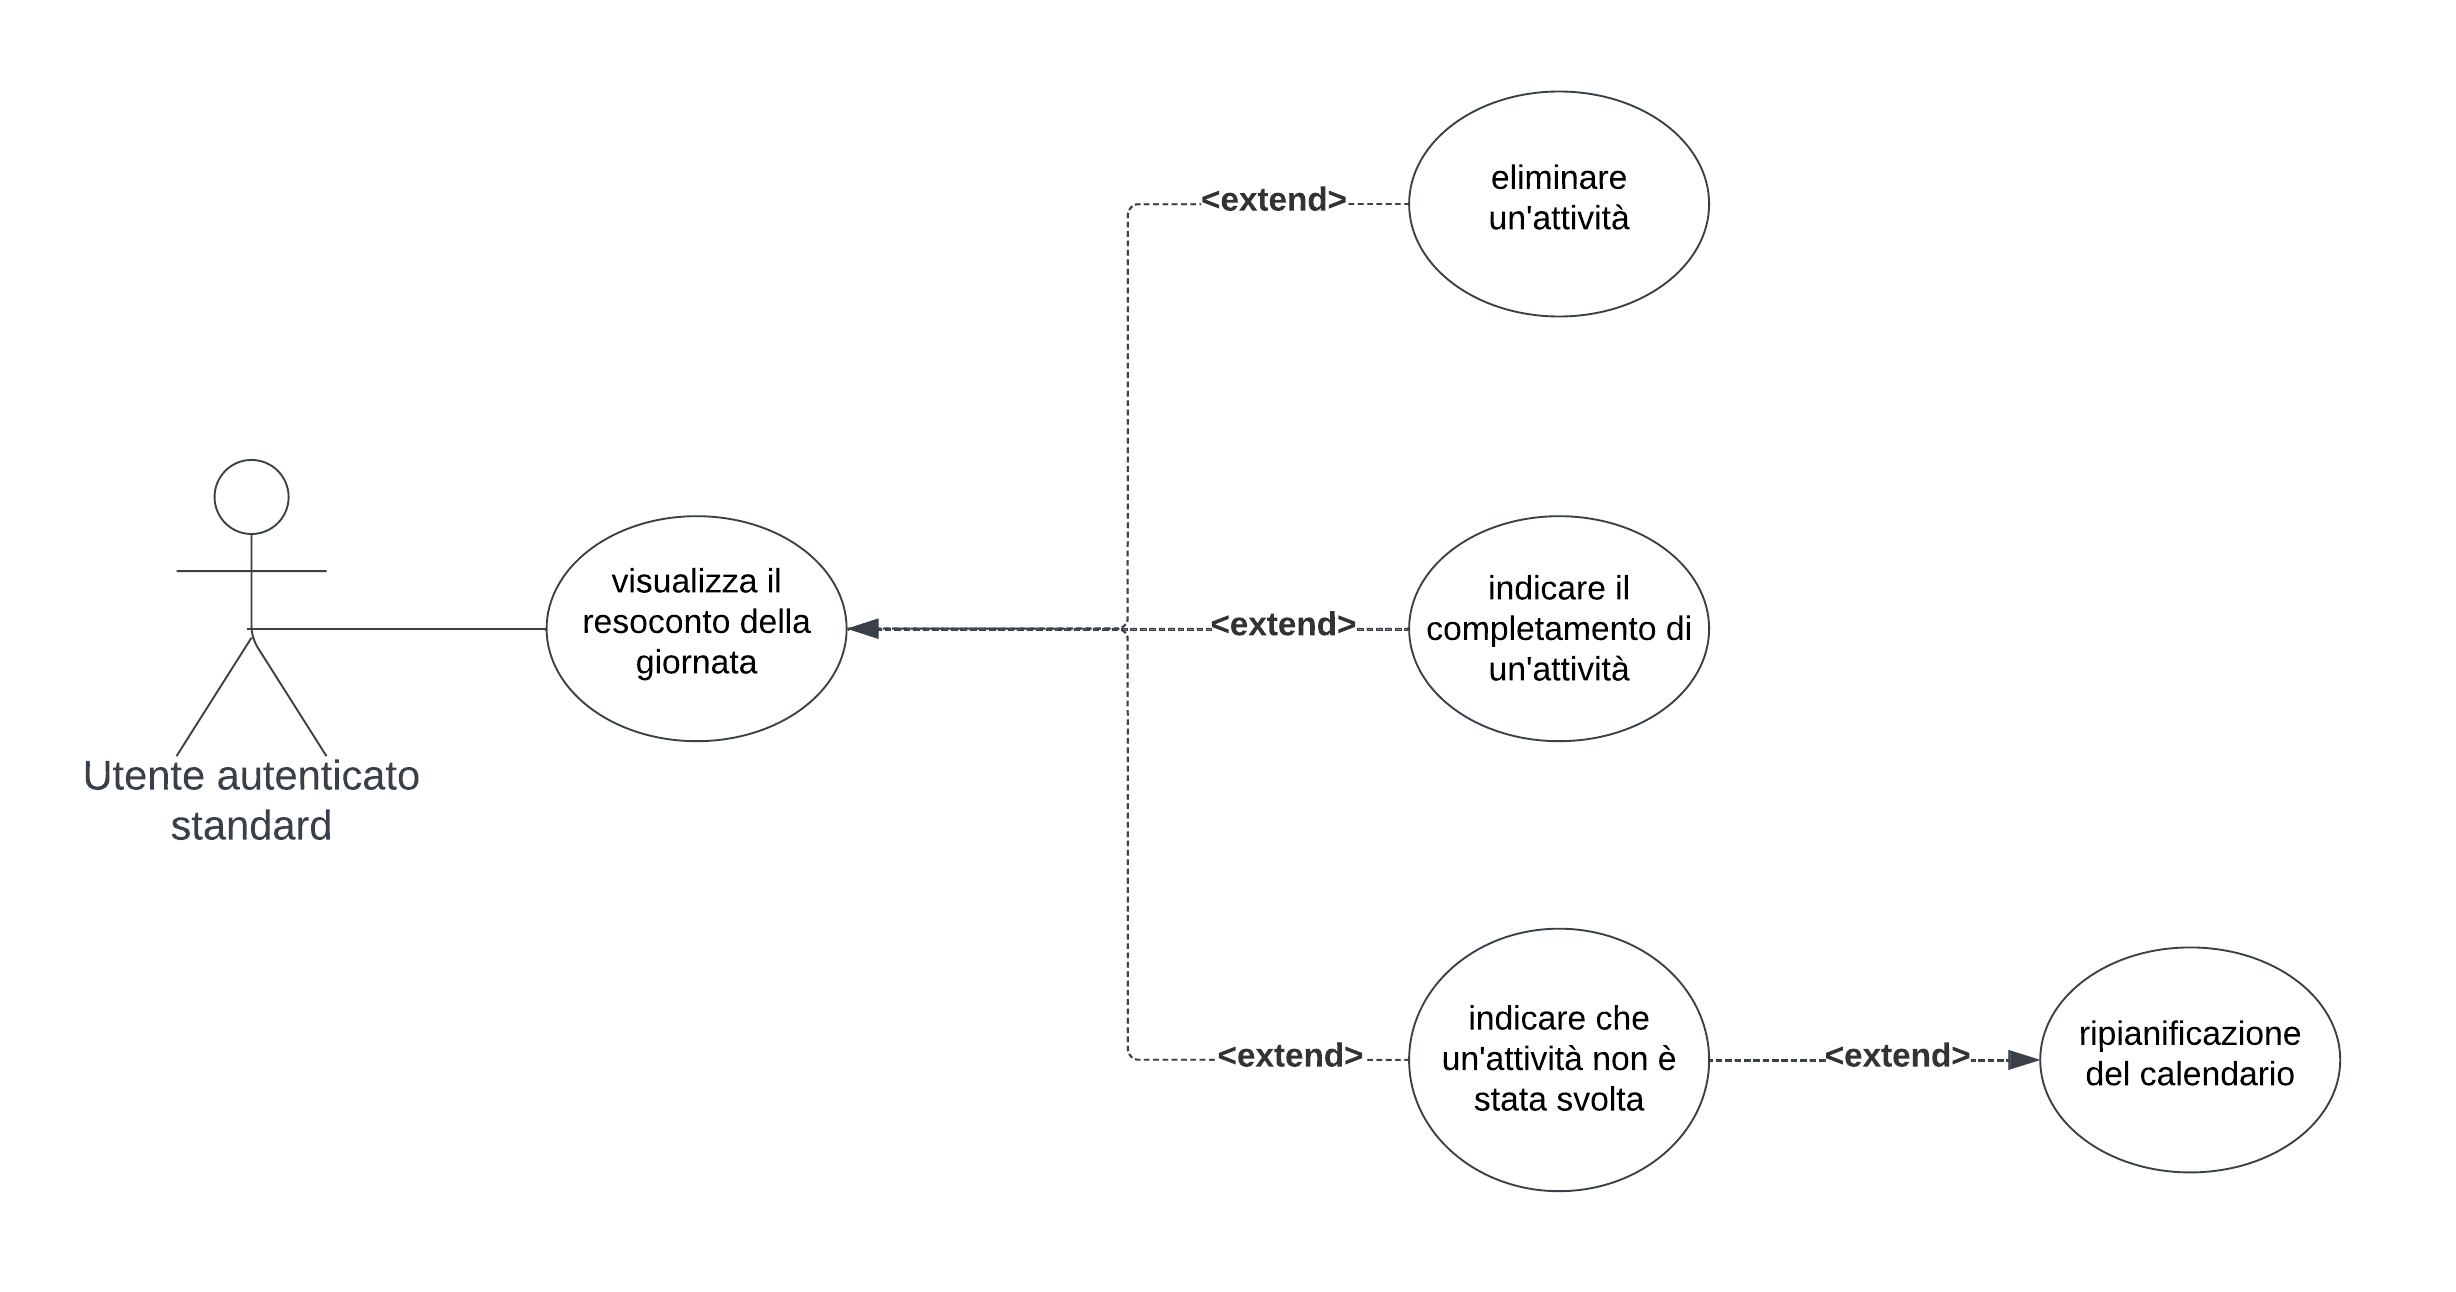
\includegraphics[width=0.7\textwidth]{img/Diagrammi/UseCases/ResocontoGiornata.png}
    \end{center}

    \textbf{Riassunto:} \\
    Questo use case descrive come l'utente autenticato standard visualizza il resoconto della giornata, dove può indicare al sistema quali attività sono state svolte e quali no. Inoltre, in questa sezione, l'utente può anche eliminare le attività. Per resoconto della giornata si intende la lista delle attività della giornata con delle loro informazioni.

    \textbf{Descrizione:}
    \begin{enumerate}
        \item Nella sezione “Attività”, l'utente autenticato standard visualizza le attività della giornata, ovvero il resoconto della giornata, con alcune loro informazioni, ovvero:
              \begin{itemize}
                  \item titolo;
                  \item descrizione;
                  \item priorità;
                  \item durata;
                  \item posizione;
                  \item difficoltà;
              \end{itemize}
        \item Dalla sezione “Stato” presente in ciascuna attività, l'utente autenticato standard può indicare lo stato dell'attività:
              \begin{itemize}
                  \item premendo sulla “spunta”, questa diventa verde, così l'utente autenticato standard indica il completamento dell'evento, ovvero che è stato svolto; \ref{uc:ExceptionModificaImpegniCompletati}
                  \item premendo sull' “orologio”, questo diventa giallo, così l'utente autenticato standard indica il non completamento dell'attività. Indicando il non svolgimento di un'attività, il sistema ripianifica il calendario per ridefinire un altro momento dove l'utente potrà svolgere questa attività non completata; \ref{uc:ExceptionRipianificazioneAttivitaLibera}
                  \item premendo sul “cestino”, questo diventa rosso, così l'utente autenticato standard indica la volonta di eliminare l'evento dal calendario.
              \end{itemize}

    \end{enumerate}



    \textbf{Exceptions:}
    \begin{enumerate}[label=\textbf{[exception \arabic{enumii}]}, ref= \textbf{[exception \arabic{enumii}]}]
        \elemento{uc:ExceptionModificaImpegniCompletati} A fine giornata di default tutti gli impegni sono posti come completati; quindi per modificare tale “stato” deve intervenire l'utente.
        \elemento{uc:ExceptionRipianificazioneAttivitaLibera} La ripianificazione dell'attività avviene se e solo se l'attività non svolta non aveva definito giorno e ora dell'impegno. Nel caso in cui fosse un evento per cui l'utente aveva definito giorno e ora dell'attività in fase di compilazione e aggiunta evento, tale attività non verrà ripianificata.
    \end{enumerate}

    \todo{nel FE ordine la lista al contrario non ha molto senso … Per @greit}





    \newpage
    \elemento[Use case “impostazione delle notifiche per evento” (\prettyref{D1-rf:Notifiche})]{uc:ImpostazioniNotifiche}


    \begin{center}
        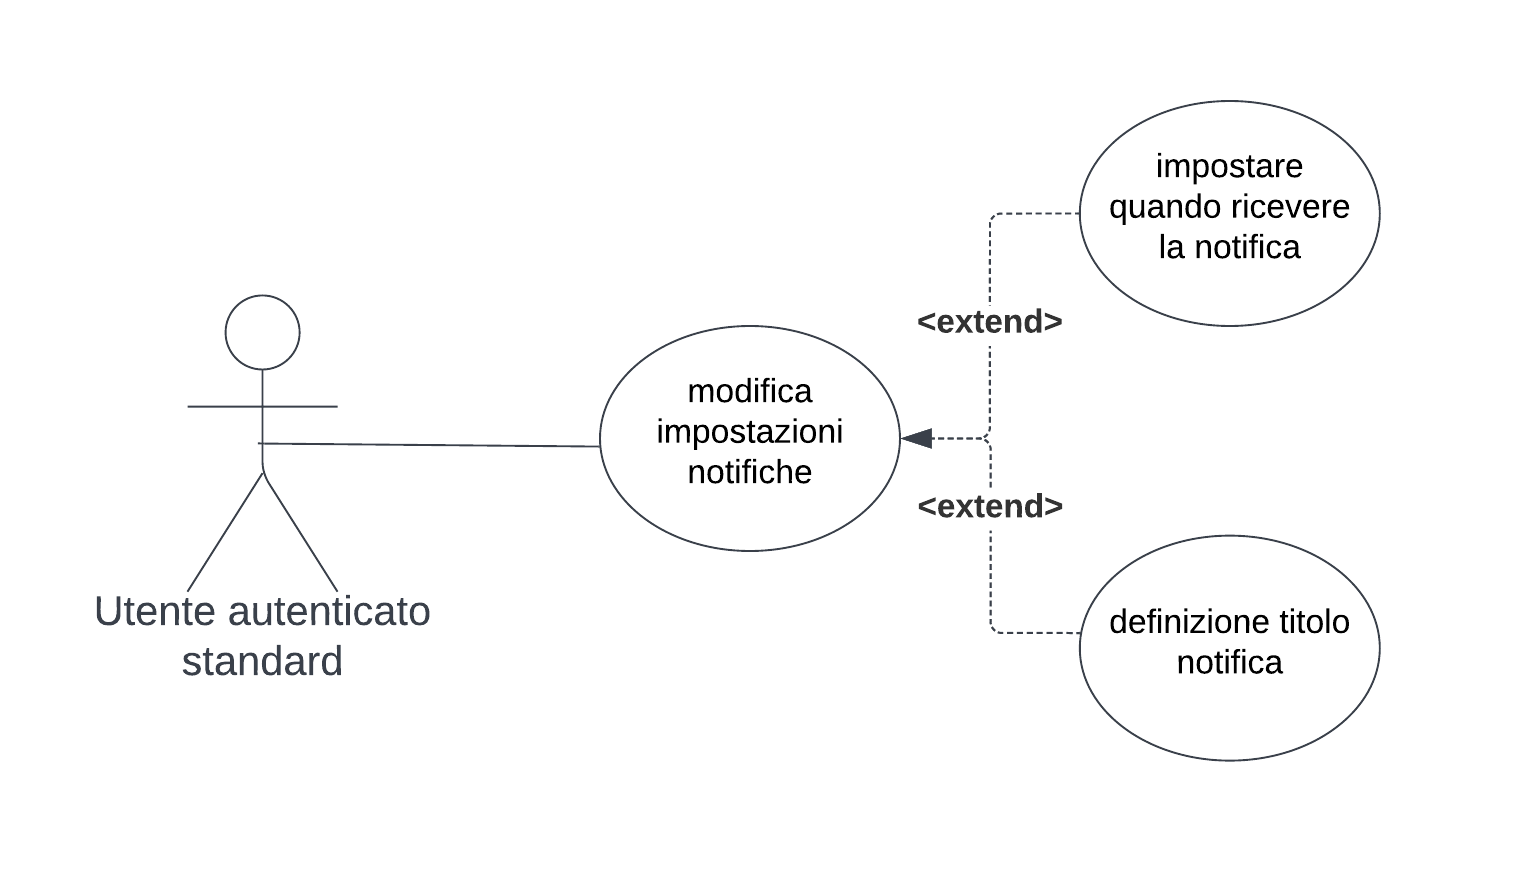
\includegraphics[width=0.7\textwidth]{img/Diagrammi/UseCases/Notifiche.png}
    \end{center}

    \textbf{Titolo:} impostazione delle notifiche per evento

    \textbf{Riassunto:} \\
    Questo use case descrive come avviene l'impostazione delle notifiche per un evento. Infatti il sistema dà la possibilità all'utente autenticato standard di personalizzare le notifiche nella fase aggiunta e di modifica dell'evento.

    \textbf{Descrizione:}
    \begin{enumerate}
        \item L'utente autenticato standard dalla schermata “Modifica/Crea Evento” visualizza il menù “Notifiche”.
        \item L'utente autenticato standard premendo sul campo “Notifiche” apre un pop-up dove può definire quando ricevere la notifica dell'evento, selezionando il campo "orario" e andando a scrivere in esso. \ref{uc:ExceptionImpostazioniNotifiche}.
        \item L'utente autenticato standard, sempre nel pop-up, può inserire il titolo della notifica che riceverà \ref{uc:ExceptionImpostazioniNotifiche} selezionando il campo "titolo" e andando a scrivere in esso.
    \end{enumerate}

    \textbf{Exceptions:}
    \begin{enumerate}[label=\textbf{[exception \arabic{enumii}]}, ref= \textbf{[exception \arabic{enumii}]}]
        \elemento{uc:ExceptionImpostazioniNotifiche} Nel caso in cui l'utente autenticato standard decidesse di non modificare i campi presenti in “Notifiche” verrà mantenuto il valore definito nelle impostazioni predefinite del calendario (\prettyref{D1-rf:ImpostazioniPredefiniteCalendario}), ovvero:
        \begin{itemize}
            \item la notifica verrà mandata tanto prima quanto indicato nell'impostazione predefinita del calendario in cui stiamo aggiungendo tale evento;
            \item la notifica avrà come titolo, il titolo dell'evento stesso.
        \end{itemize}
        \elemento{uc:ExceptionImpostazioniNotificheVuote} Nel caso in cui l'utente autenticato standard non avesse definito neanche le impostazioni delle notifiche in "Impostazioni predefinite calendario", l'utente autenticato standard non riceverà nessuna notifica per l'evento interessato.
    \end{enumerate}




    



    \newpage
    \elemento[Use case “Informazioni sull'uso del tempo” (\prettyref{D1-rf:UsoDelTempo})]{uc:InformazioniUsoDelTempo}


    \begin{center}
        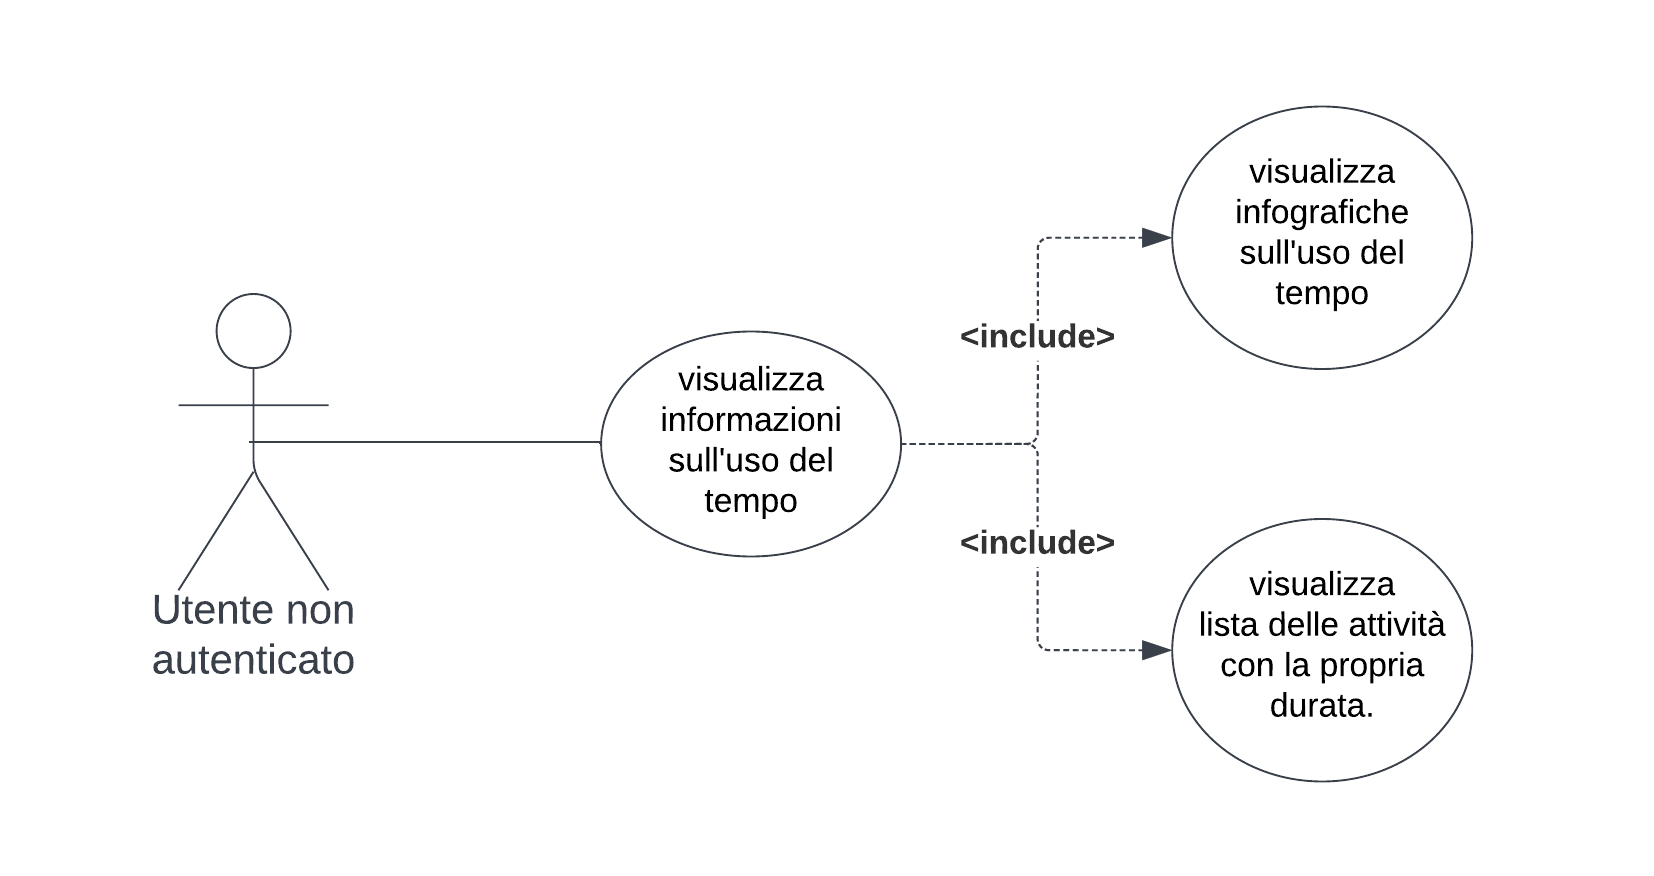
\includegraphics[width=0.7\textwidth]{img/Diagrammi/UseCases/UsoDelTempo.png}
    \end{center}

    \textbf{Titolo:} informazioni sull'uso del tempo

    \textbf{Riassunto:} \\
    Questo use case descrive come l'utente non autenticato può visualizzare dei grafici e liste esemplificative sull'uso del proprio tempo.

    \textbf{Descrizione:}
    \begin{enumerate}
        \item L'utente non autenticato dalla sezione Dashboard visualizza delle infografiche:
              \begin{itemize}
                  \item un grafico a barre dei vari eventi per ogni giorno della settimana; l'altezza delle barre corrisponde al quantitativo di ore dedicate a quell'attività. \ref{uc:ExtensionSelezioneAttivita}
                  \item una heatmap riguardo al tempo che deve essere dedicato ogni giorno per rispettare le varie deadline.
                  \item un grafico a torta delle attività. La dimensione di ciascuna attività, all'interno del grafico, e' proporzionata al tempo da spendere.
              \end{itemize}
        \item L'utente non autenticato, in questa sezione, visualizza anche una lista delle attività del proprio calendario, che è sincronizzata con il grafico a torta sopra citato, ovvero nelle due sezioni sono presenti le stesse attività con le medesime durate. \ref{uc:ExtensionSincronizzazioneGrafici} \ref{uc:ExtensionVisualizzazioneAttivita}
    \end{enumerate}

    \textbf{Extensions:}
    \begin{enumerate}[label=\textbf{[extension \arabic{enumii}]}, ref= \textbf{[extension \arabic{enumii}]}]
        \elemento{uc:ExtensionSelezioneAttivita} Selezionando un' attività dalla legenda del grafico, il grafico evidenzia l'attività selezionata in modo tale che l'utente non autenticato possa vedere più in dettaglio quando ha tale evento.
        \elemento{uc:ExtensionSincronizzazioneGrafici} La sincronizzazione tra grafico a torta e lista di attività si mantiene anche in caso di modifiche temporanee della lista di attività. Infatti premendo su un'attività, il sistema modifica la lista delle attività mostrando le sottoattività di quest'ultima e aggiornando il grafico a torta secondo la nuova lista visualizzata.
        \elemento{uc:ExtensionVisualizzazioneAttivita} Mettendo il cursore sopra ad una delle attività della lista, l'utente non autenticato visualizza evidenziata tale attività nel grafico a torta.
    \end{enumerate}



    \newpage
    \elemento[“Filtro impegni” (\prettyref{D1-rf:Filtro})]{uc:FiltroImpegni}


    \begin{center}
        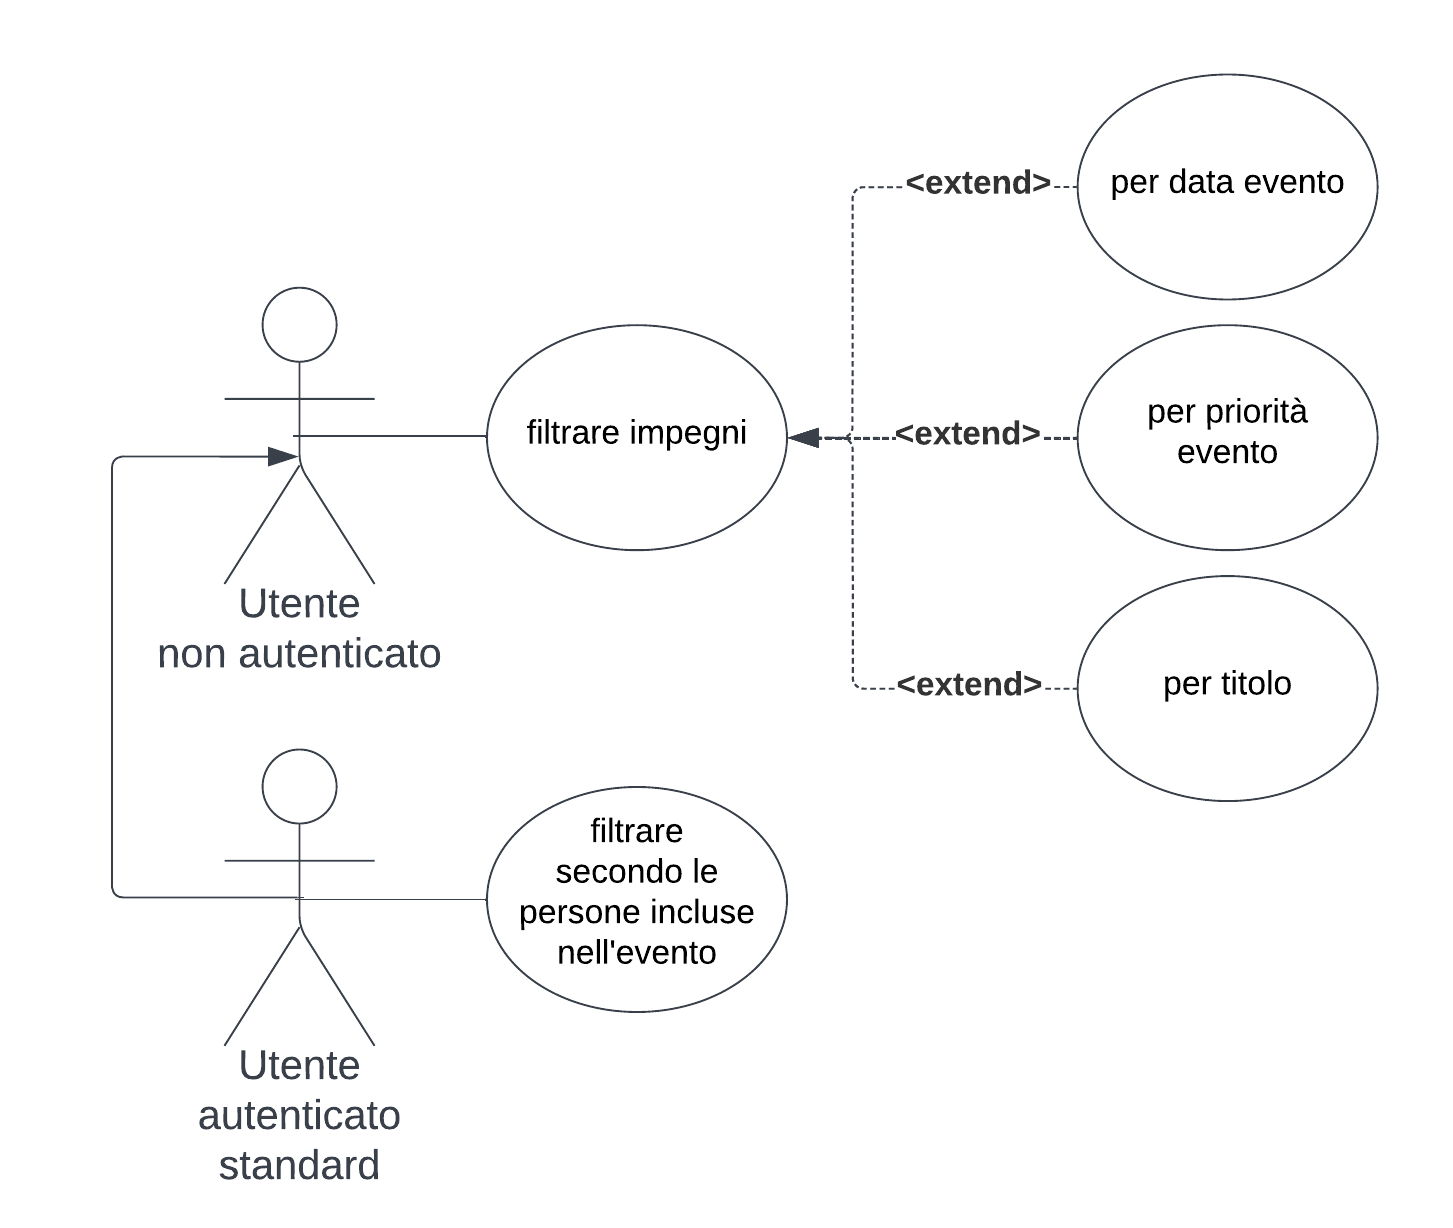
\includegraphics[width=0.7\textwidth]{img/Diagrammi/UseCases/Filtro.png}
    \end{center}
    \begin{listaPersonale2}[UC] {}
    \elemento[Use case "Filtrare impegni"] {uc:FiltroImpegniNonAutenticato}
    \textbf{Titolo:} filtrare impegni

    \textbf{Riassunto:} \\
    Questo use case descrive come l'utente non autenticato visualizza gli impegni dato un specifico filtro definito secondo alcuni criteri scelti dall'utente non autenticato.

    \textbf{Descrizione:}
    \begin{enumerate}
        \item Nelle sezione “Filtro” l'utente non autenticato può visualizzare gli impegni dato un specifico filtro definito dall'utente secondo alcuni criteri:
              \begin{itemize}
                  \item titolo evento con corrispondenza totale o parziale;
                  \item data evento;
                  \item priorità evento;
              \end{itemize}

        \item L'utente non autenticato può definire secondo quali valori dei criteri andare a filtrare gli impegni andando selezionare ciascuna casella del rispettivo criterio e andando a scrivere il valore che si preferisce in esse. Le caselle, dei vari criteri per il filtro, sono visualizzabili in questa sezione “Filtro”. \ref{uc:ExceptionNienteCriterioFiltro}
        \item Dopo aver definito i criteri degli impegni da visualizzare, l'utente non autenticato, premendo il tasto di "ricerca", visualizzerà, in un pop-up, la lista delle attività che rispettano i criteri imposti dall'utente.
    \end{enumerate}
    \elemento [Use case "Filtrare secondo le persone incluse nell'evento"]{uc:FiltroImpegniAutenticato}

    \textbf{Titolo: } Filtro secondo le persone incluse nell'evento \\
    \textbf{Riassunto: } \\ Questo use case descrive la possibilità data all'utente autenticato standard di definire un altro criterio per filtrare gli eventi del proprio calendario.\\ 
    \textbf{Descrizione: } \\ Come si può notare, data la presenza della "generalizzazione" nell'use case diagram, l'utente autenticato standard eredita dall'utente non autenticato tutti i criteri e funzionalità del filtro impegni, ma un utente autenticato standard, nella creazione o modifica di un evento, può anche definire delle persone a cui condividere tale evento. Per questo motivo, nel filtro impegni per l'utente autenticato standard è presente anche il criterio "persone incluse nell'evento". E' presente una casella che può essere selezionata per andare a scrivere al suo interno l'username degli utenti autenticati standard, di cui vogliamo trovare gli eventi che abbiamo in condivisione. 
    Dopo aver definito gli username, premendo invio, questo criterio per il filtro impegni verrà preso in considerazione e utilizzato una volta che l'utente autenticato standard premerà il tasto "ricerca" sopra citato.

    \textbf{Exceptions:}
    \begin{enumerate}[label=\textbf{[exception \arabic{enumiii}]}, ref= \textbf{[exception \arabic{enumiii}]}]
        \elemento{uc:ExceptionNienteCriterioFiltro} Nel caso in cui l'utente non andasse a definire il valore di uno o più criteri, i valori che verranno presi in considerazione per filtrare le attività sono tutti i valori che può assumere un criterio. Per esempio, se l'utente non andasse a definire il valore del criterio priorità, nel filtrare gli impegni verranno prese in considerazioni tutte le priorità, quindi da 1 a 10.
    \end{enumerate}
    \end{listaPersonale2}

    \todo{In quale sezione sarà presente il filtro impegni? Secondo me nella pagina iniziale
        Come sarà gestito? Apparirà una lista delle attività delle attività che rispettano i criteri posti, oppure questi appariranno nel calendario (schermata principale). Direi che e' da decidere
        da mettere nel FE}



    \newpage
    \todo{Creazione? Eliminazione? L'eliminazione dovremmo sistemarla ovunque}
    
    \elemento[“Creazione o modifica di un calendario” (\prettyref{D1-rf:ImpostazioniPredefiniteCalendario})]{ud:CreazioneModificaCalendario}


    \begin{center}
        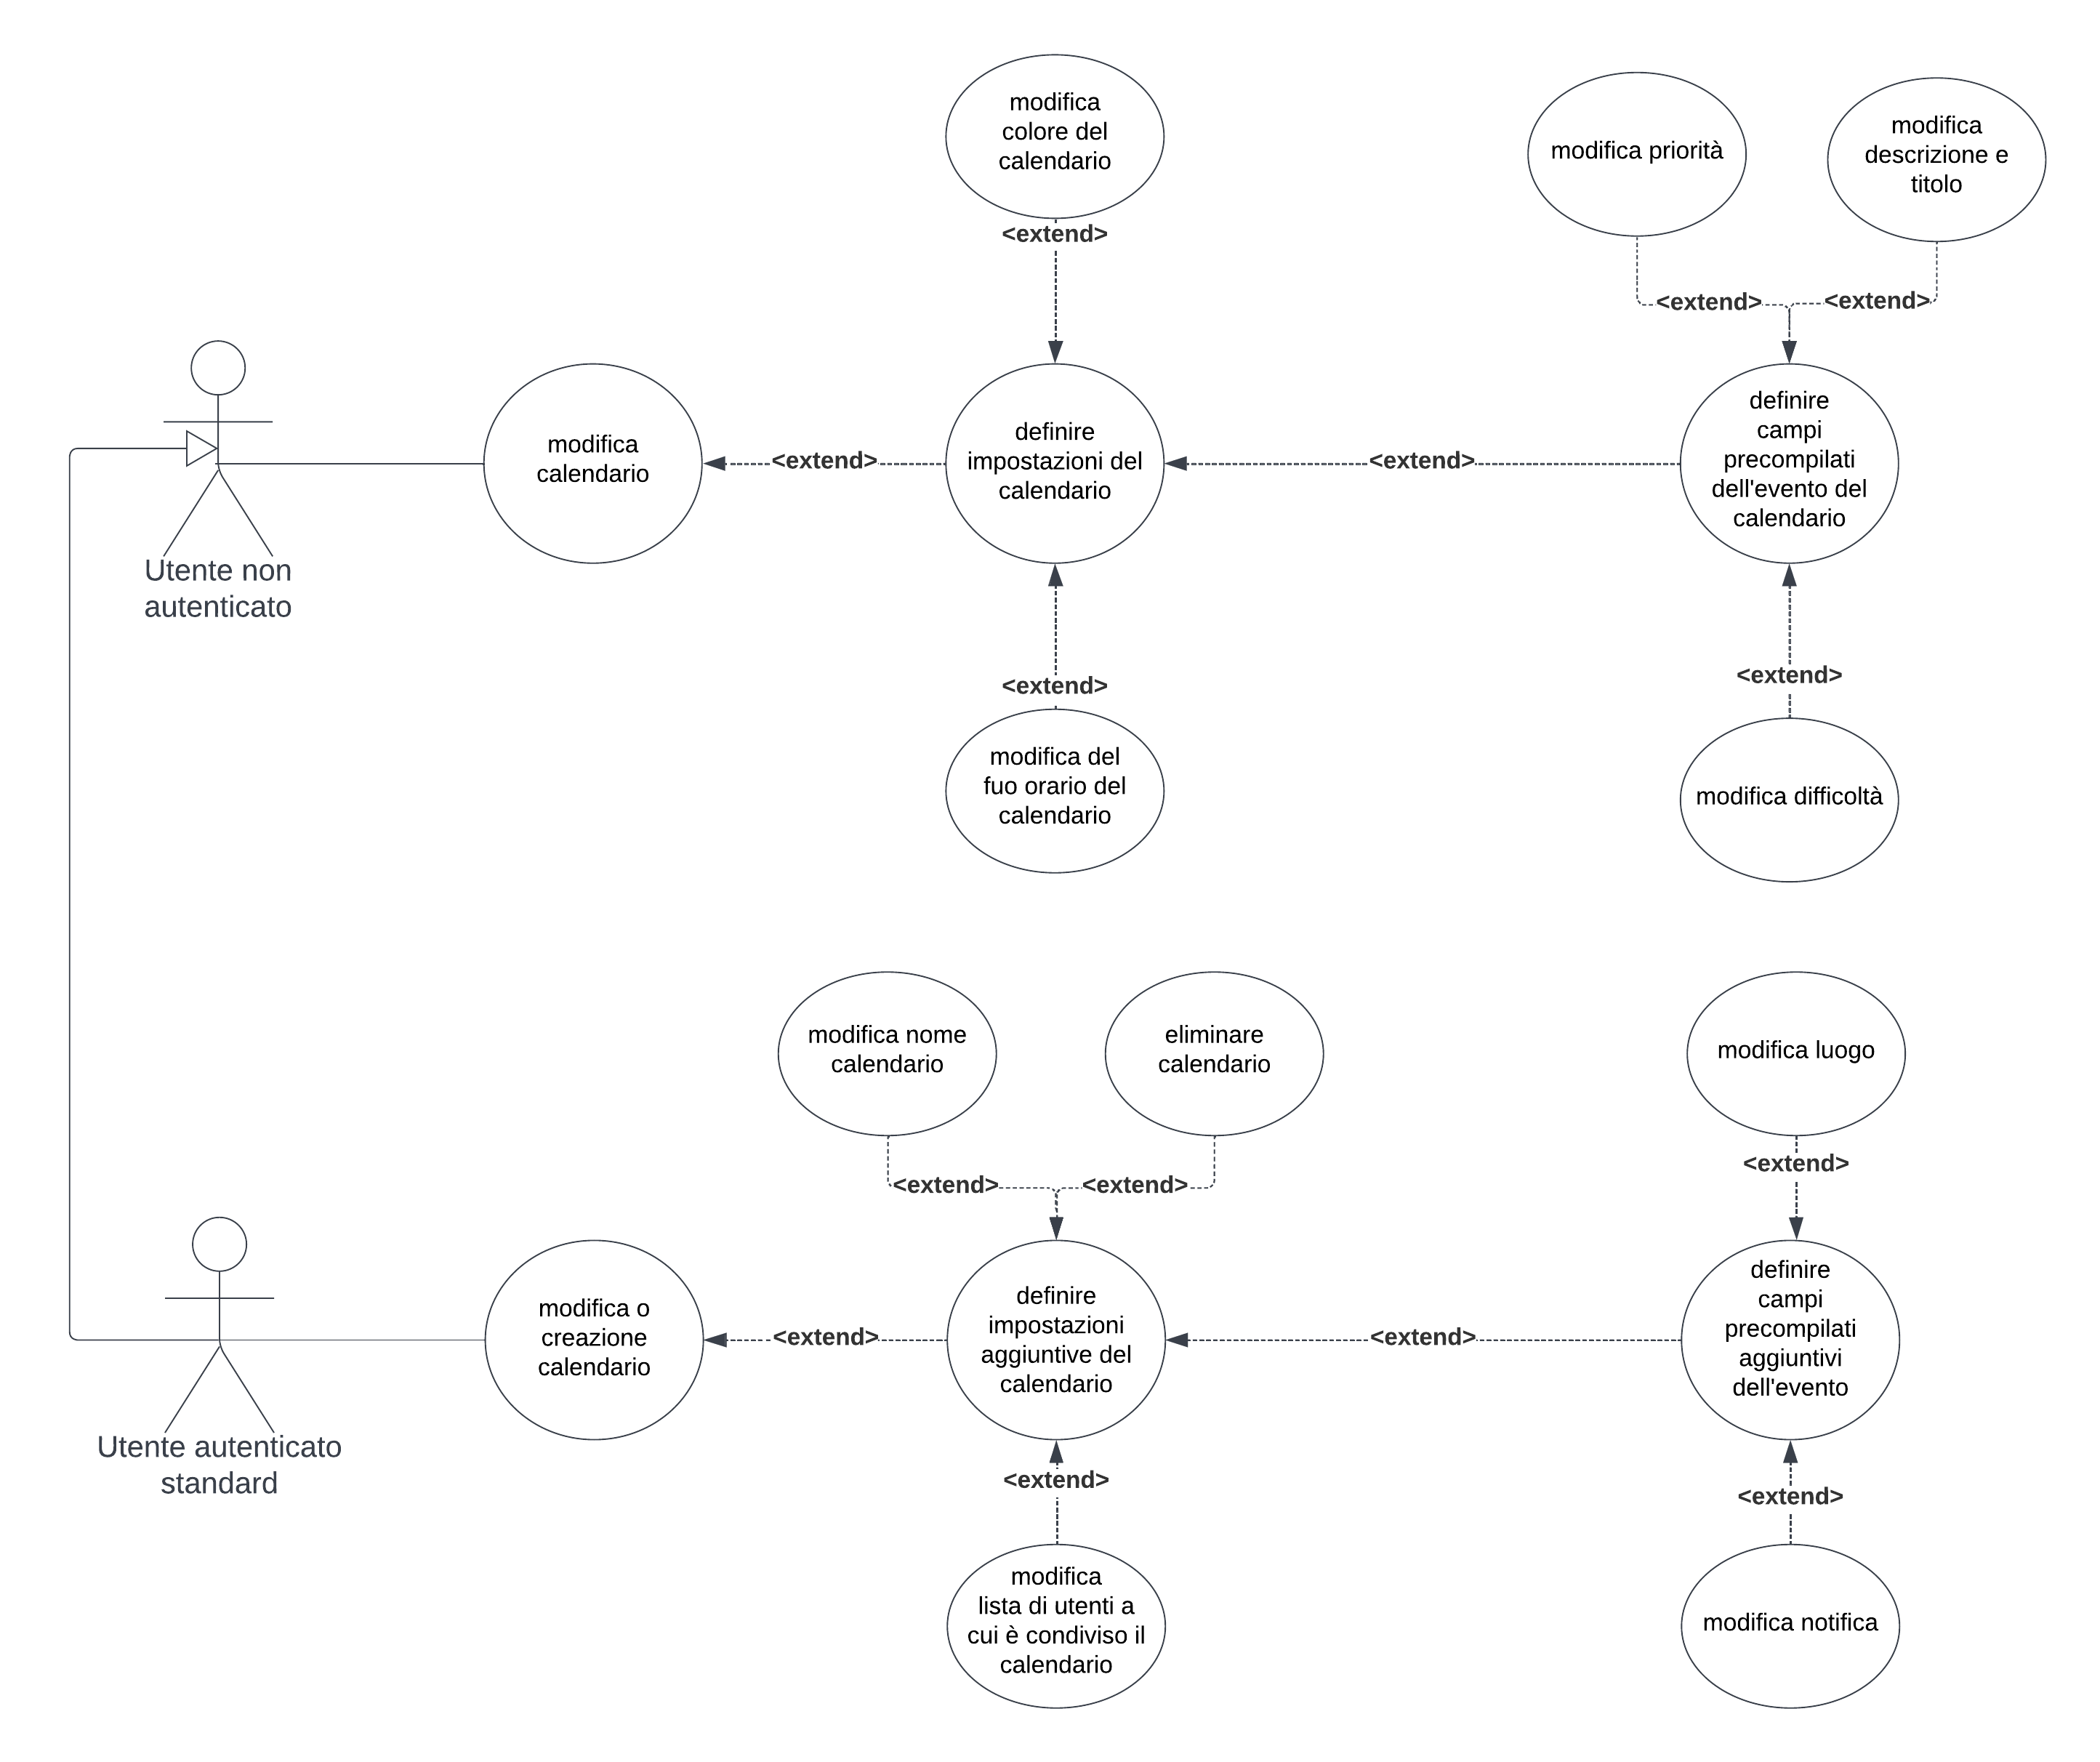
\includegraphics[width=1\textwidth]{img/Diagrammi/UseCases/ImpostazioniPredefiniteCalendario.png}
    \end{center}


    \begin{listaPersonale2}[UC] {}
        \elemento[Use case "Modifica del calendario principale"] {ud:ModificaCalendarioNonAutenticato}
        \textbf{Titolo: } modifica del calendario principale \\
        \textbf{Riassunto:} \\
        Questo use case descrive come l'utente non autenticato può andare a modificare impostazioni del calendario principale; si ricordi, che l'utente non autenticato non può avere altri calendari oltre a quello principale, per questo motivo può andare a modificare solo le impostazioni di questo. \\
        \textbf{Descrizione:} \\
        L'utente non autenticato, dalla sezione  “Impostazioni predefinite di un calendario”, può andare a modificare le impostazioni del proprio calendario principale. Nello specifico, in questa sezione sono presenti i seguenti campi che può andare a selezione e scrivere per modificare i loro valori:
                \begin{itemize}
                    \item colore del calendario, ovvero il colore con cui appariranno gli eventi appartenenti a quest'ultimo; andando a selezionare la casella "colore calendario" apparirà all'utente non autenticato la lista di colori da cui può selezionare il colore da attribuire al calendario.
                    \item fuso orario del calendario; andando a selezionare la casella "fuso orario" calendario, l'utente non autenticato può scrivere il valore del fuso orario del calendario. Si precisa che l'utilità del fuso orario di un calendario è la seguente:  se si lavora per un azienda la cui sede è in Cina, se l'azienda fissa un meeting Zoom alle loro 17, nel calendario condiviso viene inserito nell'ora corretta all'utente autenticato standard che ha impostato il fuso orario Cina, GMT+8 rispetto all'Italia, nel proprio calendario.
                \end{itemize}
        L'utente non autenticato, dopo aver modificato i campi secondo le sue preferenze, salva le modifiche fatte premendo il tasto “Salva” in fondo alla schermata di “Impostazioni predefinite di calendario”. Invece, premendo il tasto “Annulla”, le modifiche fatte non verranno salvate.
        
        \elemento[Use case "Definizione di campi precompilati di un evento del calendario principale"] {ud:DefinizioneCampiCalendarioPrincipale}
        \textbf{Titolo: } definizione di campi precompilati di un evento del calendario principale. \\
        \textbf{Riassunto: } \\ l'utente non autenticato, nella schermata "Impostazioni predefinite di calendario", può anche andare a definire dei valori con cui precompilare alcuni campi, presenti in fase di creazione di un evento da aggiungere al calendario principale. \\
        \textbf{Descrizione: } \\
        L'utente non autenticato può definire dei valori di default dei seguenti campi, presenti nella compilazione di un evento da aggiungere al calendario principale: \ref{ud:ExceptionCampiPrecompilatiCalendario}:
        \begin{itemize}
            \item priorità. E' presente una casella "priorità": l'utente non autenticato una volta selezionata tale casella, può andare a definire il valore di default della priorità.
            \item descrizione e titolo. Sono presenti le caselle descrizione e titolo: l'utente non autenticato, selezionando una alla volta le rispettive caselle, può scrivere il titolo e la descrizione di default.
            \item difficoltà, ovvero la complessità dell'evento da svolgere. E' presente una casella "priorità": l'utente non autenticato, una volta selezionata tale casella, può andare a definire il valore di default della difficoltà.
        \end{itemize}
        L'utente non autenticato salva le modifiche fatte premendo il tasto “Salva” in fondo alla schermata di “Impostazioni predefinite di calendario”. Invece, premendo il tasto “Annulla”, le modifiche fatte non verranno salvate.
        
        \elemento[Use case "creazione o modifica di un calendario personale"] {ud:CreazioneModificaCalendarioAutenticato}
        \textbf{Titolo: } Creazione o modifica di un calendario personale. \\
        \textbf{Riassunto: } \\  Questo use case descrive la possibilità dell'utente autenticato standard, di poter andare a creare o modificare un proprio calendario. Si può vedere dall'use case che è presente una "generalizzazione" che indica il fatto che l'utente autenticato standard eredita dall'utente non autenticato le sue funzionalità di modifica di un calendario. Il calendario che si vuole modificare, in questo caso, può anche non essere quello principale, in quanto l'utente autenticato standard può creare più calendari personali. Quindi questo use case ha l'obiettivo di mostrare quali funzionalità aggiuntive abbia l'utente autenticato standard nella creazione o modifica di una calendario rispetto all'utente non autenticato. \\ 
        \textbf{Descrizione: } 
        \begin{enumerate}
            \item L'utente autenticato standard, oltre alla possibilità sopra citate per l'utente non autenticato, ha ulteriori altre funzionalità quando modifica o crea un calendario, ovvero:
            \begin{itemize}
                \item impostazioni aggiuntive per i calendari;
                \item creazione o modifica di più calendari personali;
                    \todo{Quindi un Utente demo non ha i campi precompilati? Sì li ha ben, sopra li ho definiti, questi sono "aggiuntivi"}
            \end{itemize}
            \item Nella schermata di "Crea Calendario", sezione a cui accede l'utente autenticato standard quando vuole andare a creare un nuovo calendario personale, o nella schermata "Impostazioni predefinite di calendario", sezione a cui accede l'utente autenticato standard per andare a modificare le impostazioni di un proprio calendario, l'utente autenticato standard può andare a definire delle impostazioni riguardanti al calendario che sta creando o modificando, ovvero:
                \begin{itemize}
                    \item tutti i campi già presenti per la modifica del calendario principale per un utente non autenticato (\ref{ud:ModificaCalendarioNonAutenticato});
                    \item persone a cui è condiviso il calendario. Si ricordi che il calendario principale non può essere condiviso, se non per alcuni eventi che lo formano. E' presente una casella che può essere selezionata per andare a scrivere al suo interno l'username degli utenti autenticati standard, a cui vogliamo condividere tale calendario. 
                    Dopo aver definito gli username, premendo invio, questa modifica verrà presa in considerazione per la creazione o modifica del calendario, una volta che l'utente autenticato standard premerà il tasto "salva" sotto citato.
                    \item il nome del calendario che si sta creando o modificando. E' presente una casella "nome calendario": l'utente autenticato standard una volta selezionata tale casella, può andare a scrivere il nome del calendario, che verrà utilizzato nel caso in cui, alla fine della procedura di creazione o modifica, l'utente autenticato standard premerà il tasto "salva" sotto citato.               
                    \item eliminare il calendario che si sta modificando. E' presente un tasto "elimina calendario", che premuto, farà apparire un pop-up con un bottone "elimina definitivamente calendario". Una volta che l'utente autenticato standard premerà anche questo bottone, il calendario, di cui stiamo modificando le impostazioni in "Impostazioni predefinite calendario", viene eliminato. 
                \end{itemize}
            L'utente non autenticato salva le modifiche fatte premendo il tasto “Salva” in fondo alla schermata di “Impostazioni predefinite di calendario”. Invece, premendo il tasto “Annulla”, le modifiche fatte non verranno salvate.
            \end{enumerate}
        
        \elemento[Use case "Definizione di campi precompilati di un evento di un calendario personale"] {ud:DefinizioneCampiCalendarioPersonale}
        \textbf{Titolo: } definizione di campi precompilati di un evento di un calendario personale. \\
        \textbf{Riassunto: } \\ L'utente autenticato standard, nelle "Impostazioni predefinite di calendario" o nella schermata "Crea calendario", può anche andare a definire dei valori con cui precompilare alcuni campi, presenti in fase di creazione di un evento da aggiungere al calendario a cui appartiene tale evento. L'utente autenticato standard eredita dall'utente non autenticato i campi che quest'ultimo può definire, ma ha degli ulteriori campi in quanto, come già scritto, ha delle funzionalità in più in fase di creazione di un evento. \\
        \textbf{Descrizione: } \\
        \begin {enumerate}
            \item L'utente autenticato standard, trovandosi nelle "Impostazioni predefinite di calendario" o nella schermata "Crea calendario", può definire i seguenti valori con cui verranno precompilati i corrispettivi campi in fase di creazione di un evento, appartenente al calendario di cui si stanno definendo le impostazioni: \ref{ud:ExceptionCampiPrecompilatiCalendario}
            \begin{itemize}
                \item tutti i campi già presenti per la definizione di valori di default nella compilazione di un evento da parte dell'utente non autenticato (\ref{ud:DefinizioneCampiCalendarioPrincipale});
                \item luogo dove si terrà l'evento;
                \item quando ricevere la notifica dell'evento;
                \item titolo della notifica dell'evento.
            \end{itemize}
            \item L'utente autenticato standard, così, può creare o modificare il calendario premendo il tasto “Salva” che si trova in fonda alla schermata. L'utente può annullare l'azione premendo il tasto “Annulla” che trova sempre in fondo alla schermata di “Crea Calendario”.
        \end{enumerate}
        \textbf{Exceptions:}
        \begin{enumerate}[label=\textbf{[exception \arabic{enumiii}]}, ref= \textbf{[exception \arabic{enumiii}]}]
            \elemento{ud:ExceptionCampiPrecompilatiCalendario} Nel caso in cui l'utente non modificasse uno o più campi, nella compilazione per l'aggiunta di un evento l'utente non visualizzerà precompilati i campi non modificati nelle “Impostazioni predefinite di un calendario”.
        \end{enumerate}
        

        

        \todo{(L'utente autenticato standard deve selezionare il calendario, di cui vuole modificare le impostazioni, dalla lista dei propri calendari, presente nella parte sinistra di questa schermata.)Non e' troppo dettagliato? Si credo che si possa togliere, l'unica cosa è che forse questa cosa della selezione di un calendario andrebbe nella componente}


    \end{listaPersonale2}




    \newpage
    \elemento[Use case “Impostazioni account” (\prettyref{D1-rf:ImpostazioniAccount})]{uc:ImpostazioniAccount}

    \begin{center}
        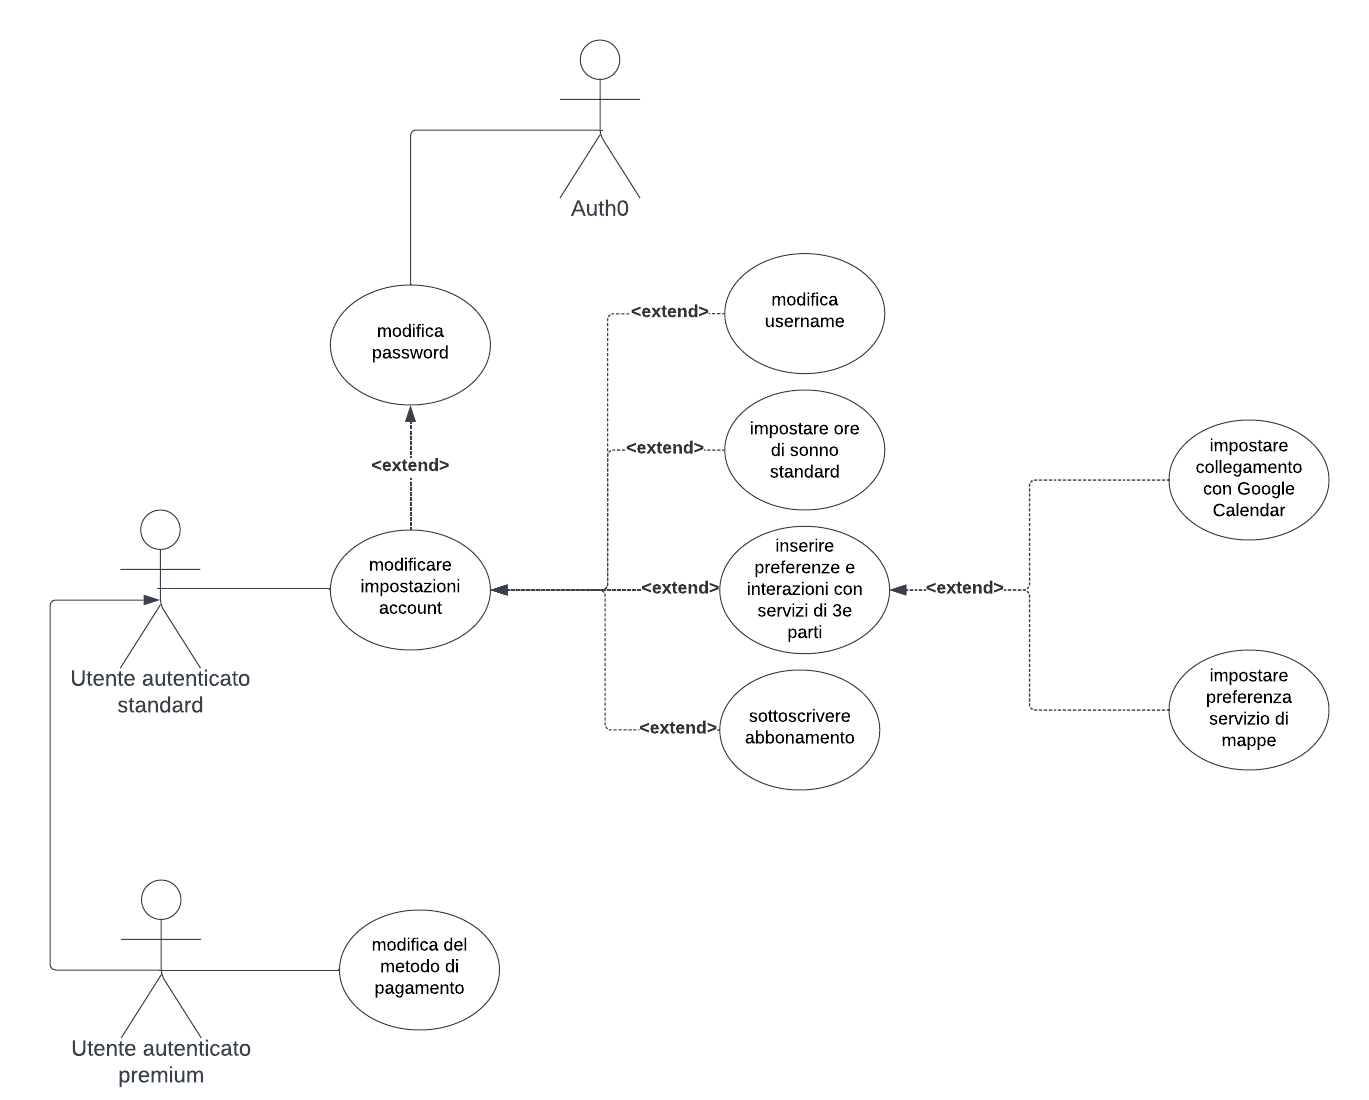
\includegraphics[width=0.75\textwidth, height = 0.35\textheight]{img/Diagrammi/UseCases/ImpostazioniAccount.png}
        Si prega di zoomare a piacere per di poter leggere bene le varie parti dell'use case
    \end{center}
    Per andare a descrivere questo use case si è deciso di utilizzare uno State Machine Diagram con swimlanes a discapito della descrizione in italiano, in quanto in questo use case sono presenti delle scelte che possono essere effettuate dall'utente autenticato standard o autenticato premium. Inoltre, non si è diviso l'Activate Diagram in due parti, a seconda della tipologia di account, in quanto se ci fossero due diagrammi, questi avrebbero molto ridondanze. Infatti, come si può notare dall'Use Case Diagram, l'utente autenticato premium presenta le stesse funzionalità di quello autenticato premium, quest'ultimo ha anche delle funzionalità aggiuntive. Al posto, quindi di fare due diagrammi, si è preferito farne uno che presente il controllo per poter sapere se l'utente autenticato in questione è o standard o premium in modo tale da fornire le giuste funzionalità.
    Infine, in quanto gli use case "interagire con Google Calendar" e "sottoscrivere abbonamento" presentano delle procedure da analizzare più dettagliatamente, si è deciso di fare dei sotto use case a parte, che entrano molto di più nel merito delle funzionalità.
    \newpage
    \textbf{Diagramma:}
    \begin{center}
        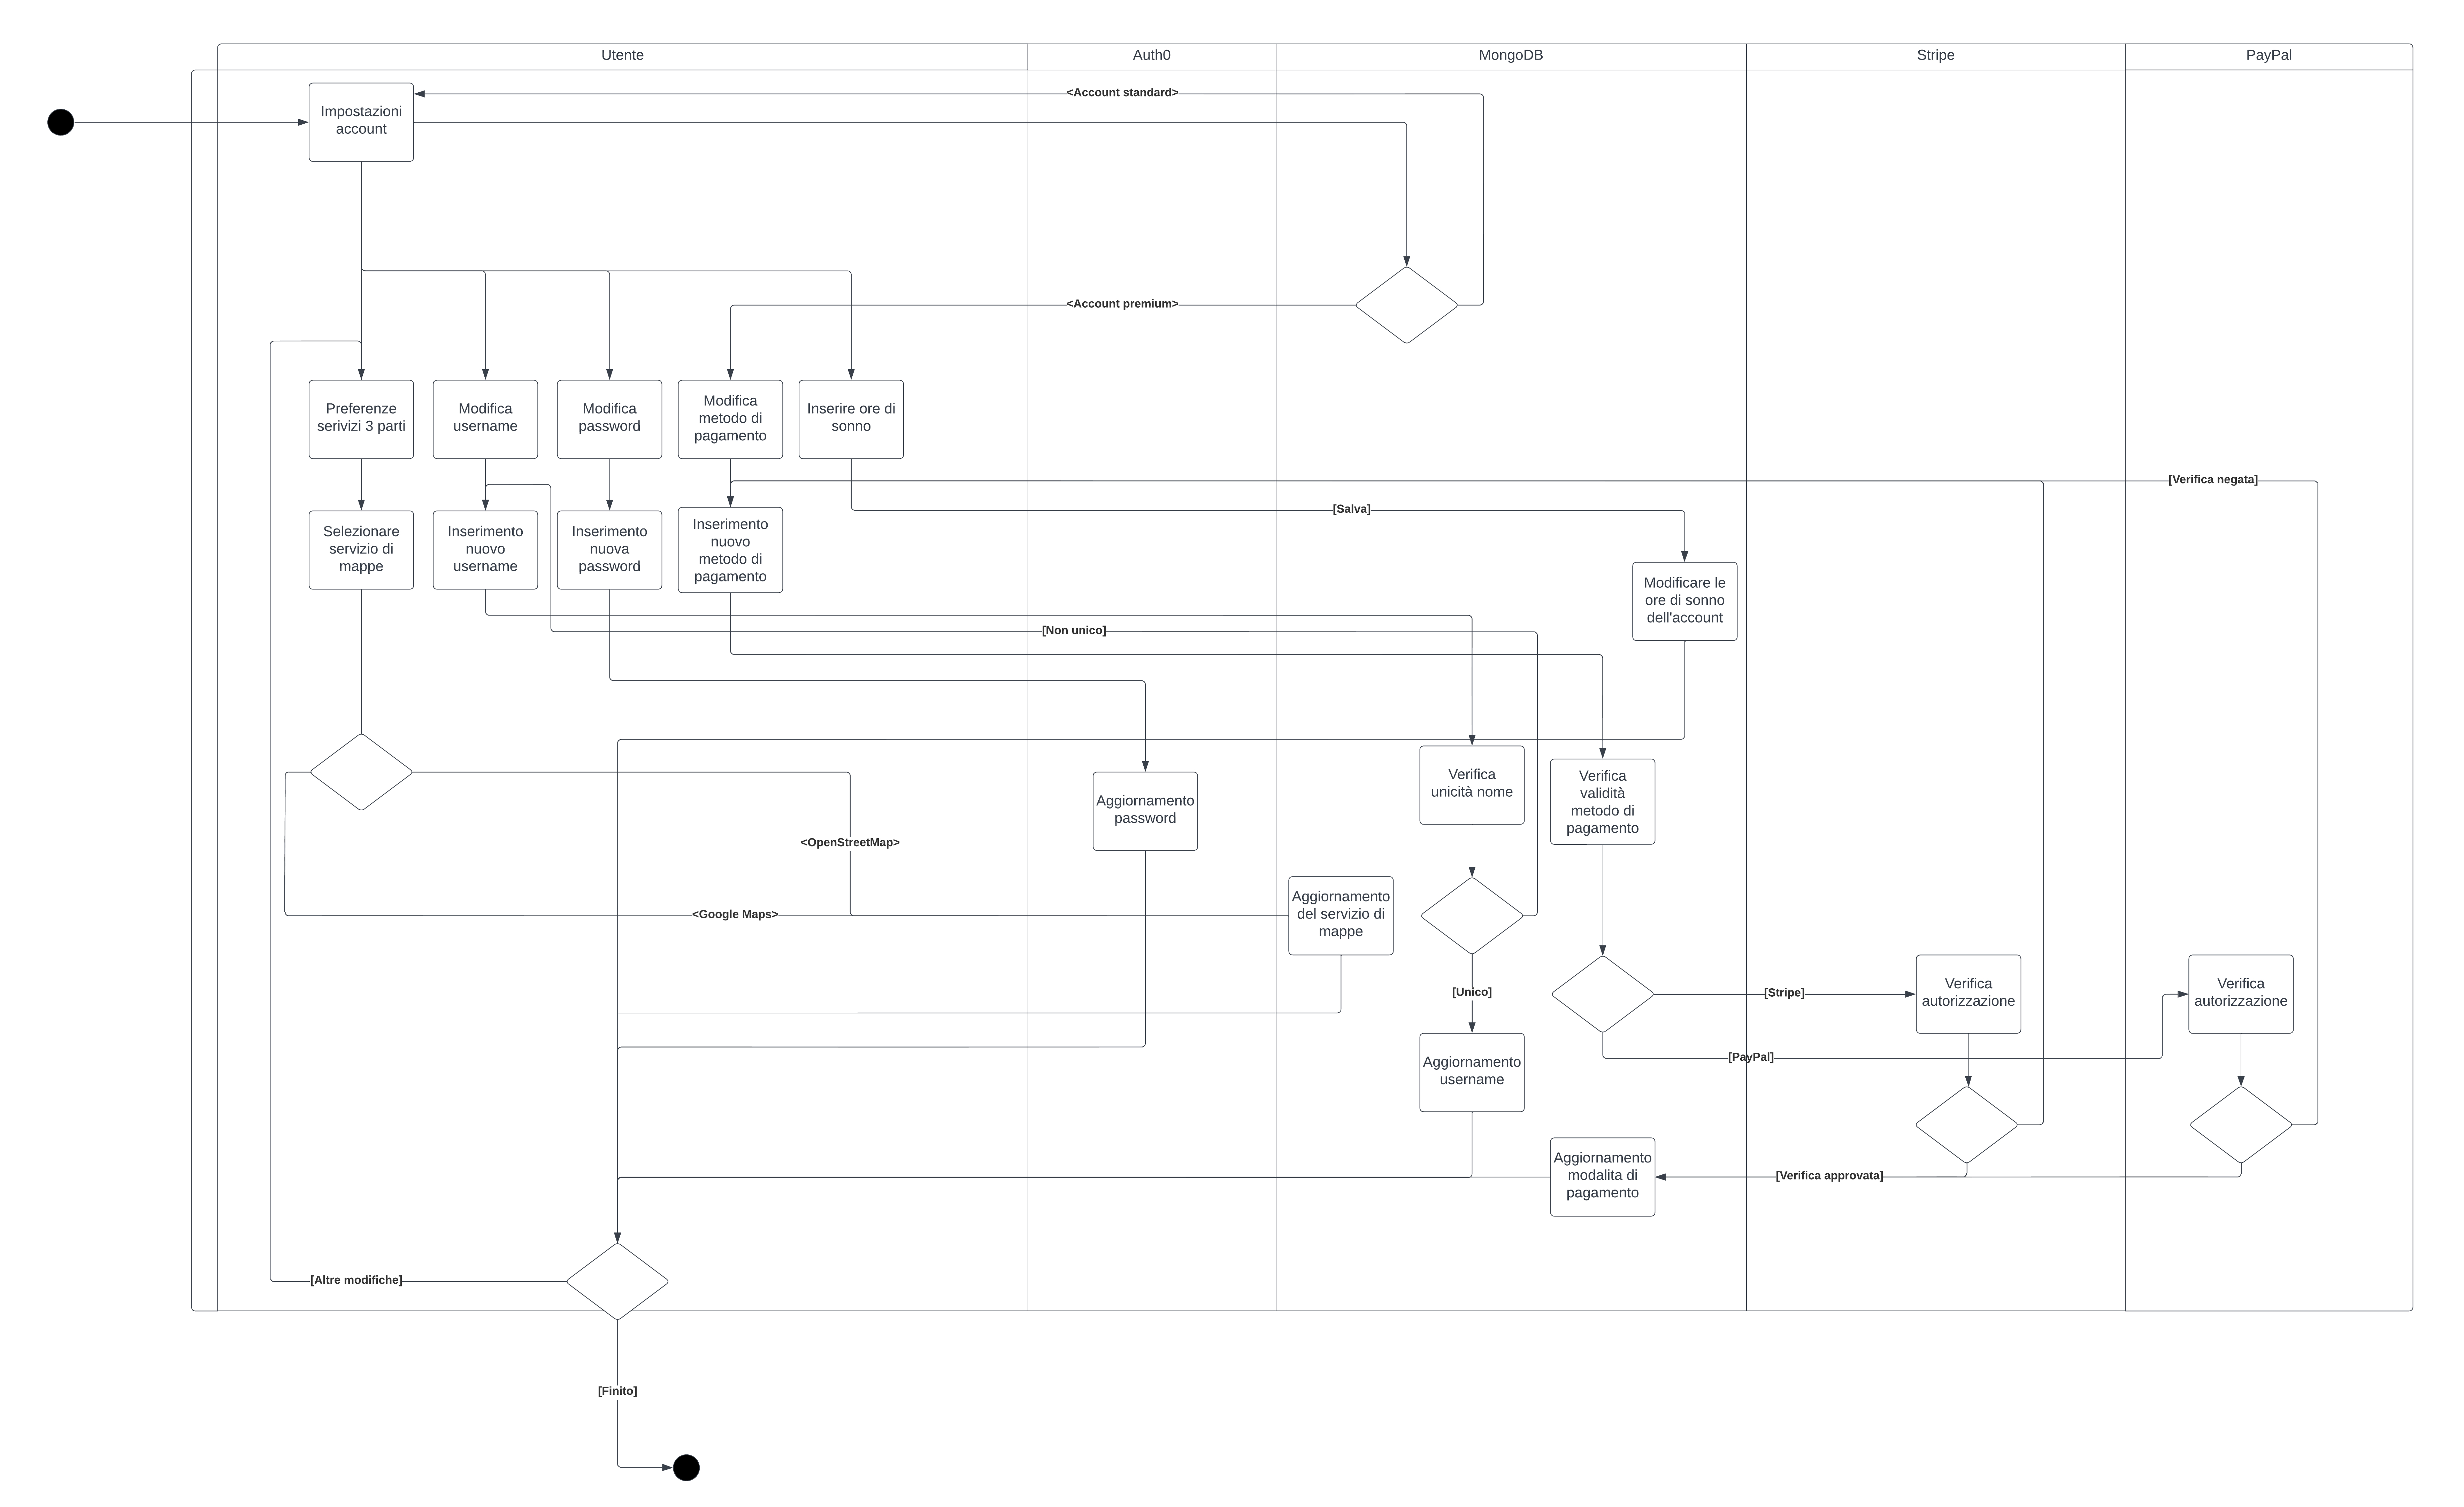
\includegraphics[width=1.1\textwidth]{img/Diagrammi/DS/DS_ImpostazioneAccount.png}
        Si prega di zoomare a piacere per poter leggere bene le varie parti del diagramma
    \end{center}
    \begin{listaPersonale2}[UC] {}
        \elemento[Use case “Sottoscrizione all'account premium” (\prettyref{D1-rf:PagamentoUtentePremium})]{uc:SottoscrizioneAccountPremium}

        \begin{center}
            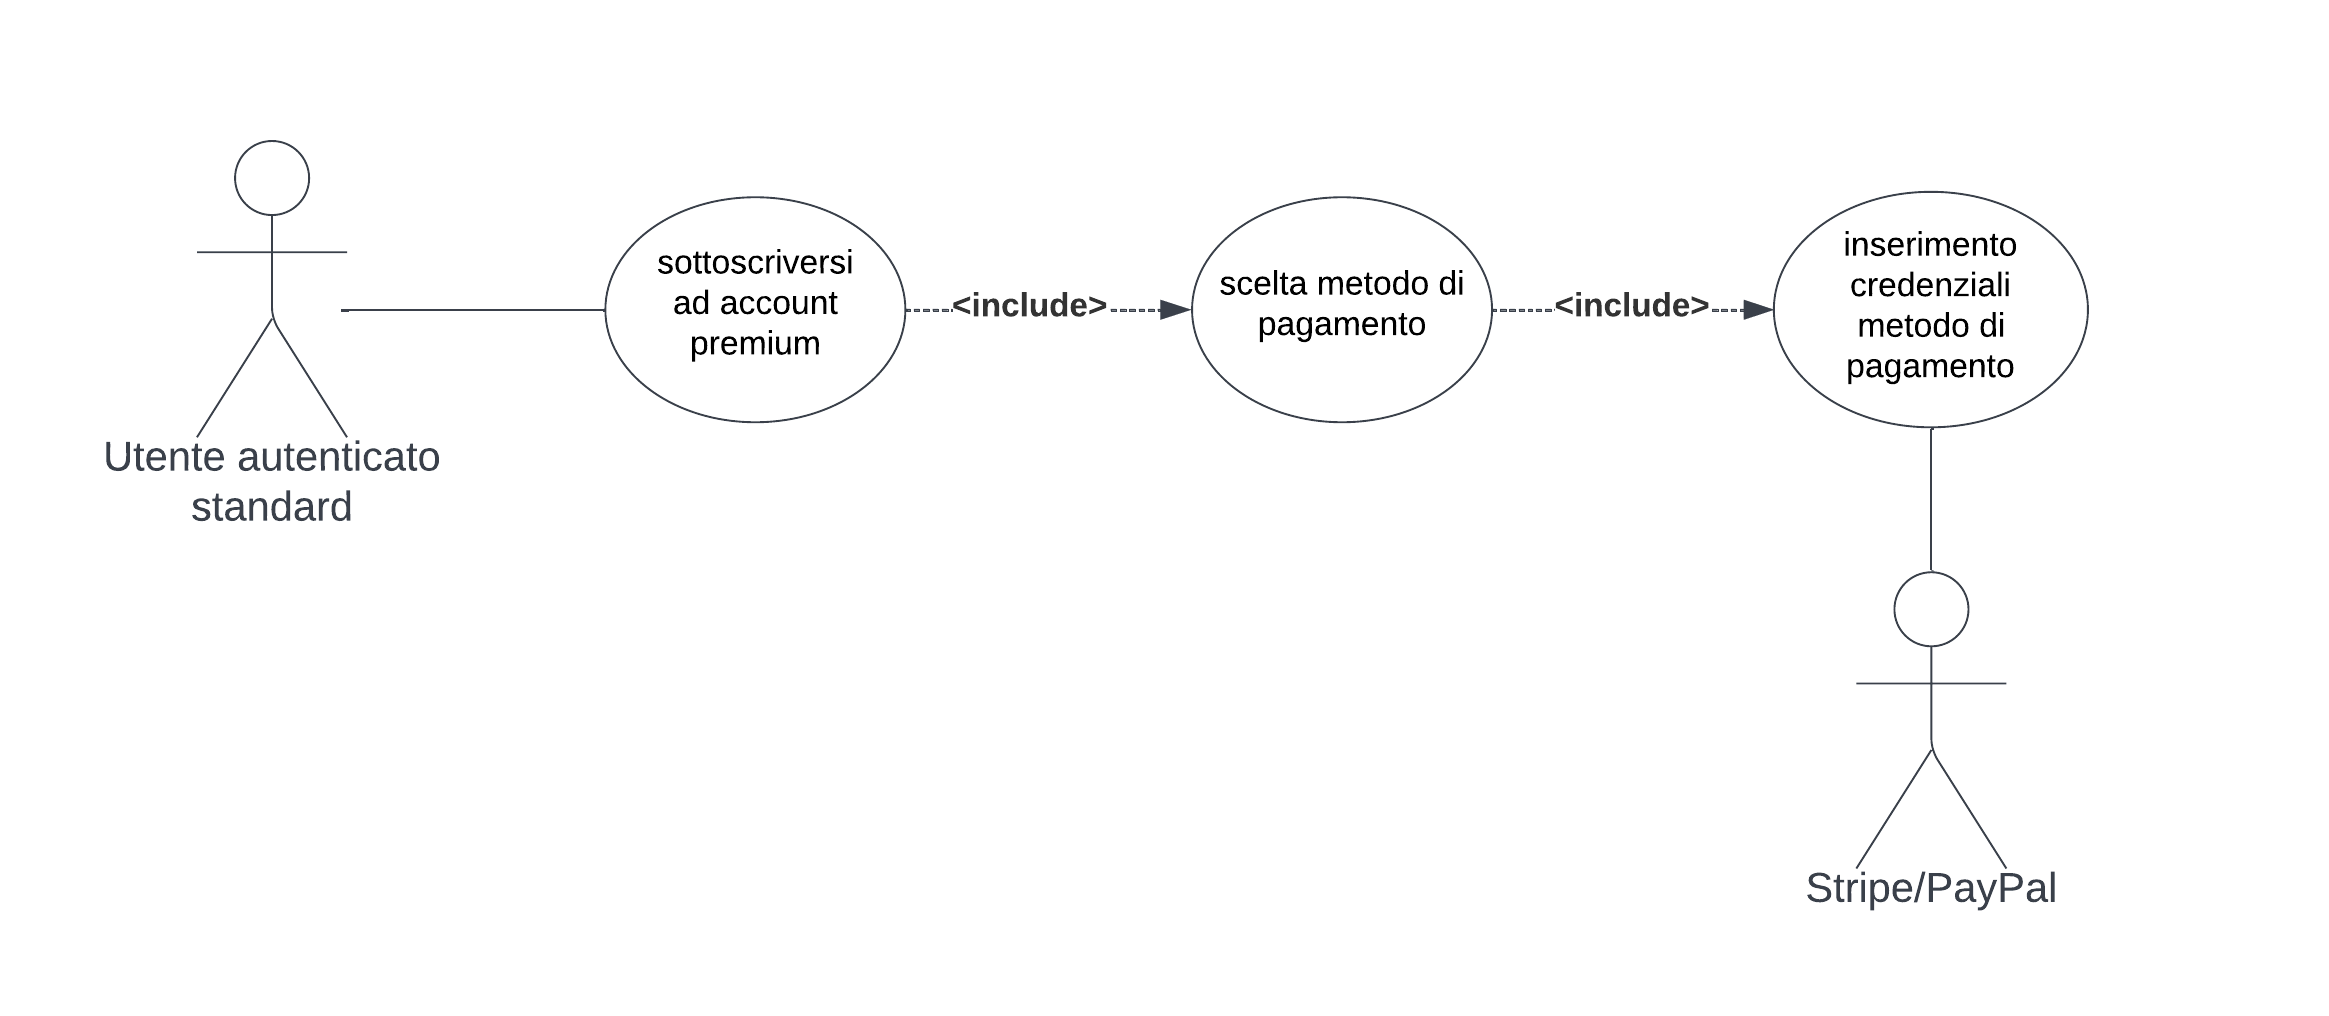
\includegraphics[width=0.7\textwidth]{img/Diagrammi/UseCases/UtentePremium.png}
        \end{center}


        \textbf{Titolo:} sottoscrizione all'account premium.

        \textbf{Riassunto:} \\
        Questo use case descrive come avviene la sottoscrizione all'account premium mediante un abbonamento a pagamento.
        Questo use case è una specifica dell'use case "Impostazioni Account" in quanto la procedura di sottoscrizione all'account premium richiede una maggiore dettagliatezza e, per questo motivo, si è deciso di fare un use case a parte.

        \textbf{Descrizione:}
        \begin{enumerate}
            \item L'utente autenticato standard, nella sezione “impostazioni account”, preme il tasto il campo: “Abbonarsi”.
            \item Una volta selezionato questo campo, l'utente autenticato standard dovrà scegliere tra due possibili metodi di pagamento predefiniti: Stripe o PayPal. L'utente autenticato standard sceglie il metodo di pagamento preferito, selezionando la sua icona, e premendo il tasto "Avanti".
            \item Dopo aver scelto uno dei metodi di pagamento, l'utente autenticato standard verrà indirizzato nella pagina del metodo di pagamento selezionato, dove dovrà inserire le proprie credenziali riguardanti il suo account del sistema esterno di pagamento. \ref{uc:ExceptionCredenzialiSistemaDiPagamento}
            \item Una volta che l'utente autenticato standard avrà inserito queste credenziali, l'utente autenticato standard avrà aggiunto correttamente al suo account il metodo di pagamento dell'abbonamento.
            \item L'abbonamento all'account premium, a questo punto, partirà automaticamente con un costo mensile di 15 euro. Ogni mese il pagamento verrà fatto in maniera automatica mediante il metodo di pagamento inserito \ref{uc:ExceptionPagamentoNonValido}, che può essere modificato in “Impostazioni Account”. 
            \item L'account premium può essere disabilitato, in ogni momento, da “Impostazioni Account” premendo sul tasto "Modifica metodo di pagamento": una volta premuto questo tasto, invece che andare a scegliere un nuovo metodo di pagamento per l'abbonamento, non si deve andare a definire nessuna scelta premendo subito il tasto "Avanti", così automaticamente il sistema, in assenza di scelta del metodo di pagamento, annullerà l'abbonamento a fine del periodo di sottoscrizione (ovvero quando finisce il mese di sottoscrizione).
        \end{enumerate}

        \todo{Forse dovremmo fare un requisito funzionale per disabilitare account premium?! Si dovremmo metterlo, ma a quel punto dovremmo fare anche un use case + descrizione}

        \textbf{Exceptions:}
        \begin{enumerate}[label=\textbf{[exception \arabic{enumiii}]}, ref= \textbf{[exception \arabic{enumiii}]}]
            \elemento{uc:ExceptionCredenzialiSistemaDiPagamento} L'inserimento delle credenziali andrà avanti finché l'utente non inserirà delle credenziali corrette del sistema esterno del metodo di pagamento scelto. Infatti l'utente autenticato standard va avanti con la procedura della sottoscrizione solo una volta che ha inserito delle credenziali corrette.
            \elemento{uc:ExceptionPagamentoNonValido} In caso il saldo dell'utente presso la piattaforma di pagamento selezionata non sia sufficiente per coprire il costo dell'abbonamento, l'abbonamento stesso si interromperà e tutte le funzioni premium a esso collegate non verranno più rese disponibili fino al prossimo pagamento.
        \end{enumerate}
        \todo{Qua c'è un problema non possiamo mettere la sottoscrizione dalle impostazioni Account sennò dopo dobbiamo andare a modificare in realtà impostazioni account e il suo state diagram. Qua in realtà ne avevamo anche parlato con il prof che ha detto che va bene, andiamo a specificare che questo use case è una specifica di impostazioni account.}


        \elemento[Use case “interagire con Google Calendar” (\prettyref{D1-rf:GoogleCalendar})]{uc:GoogleCalendar}


        \begin{center}
            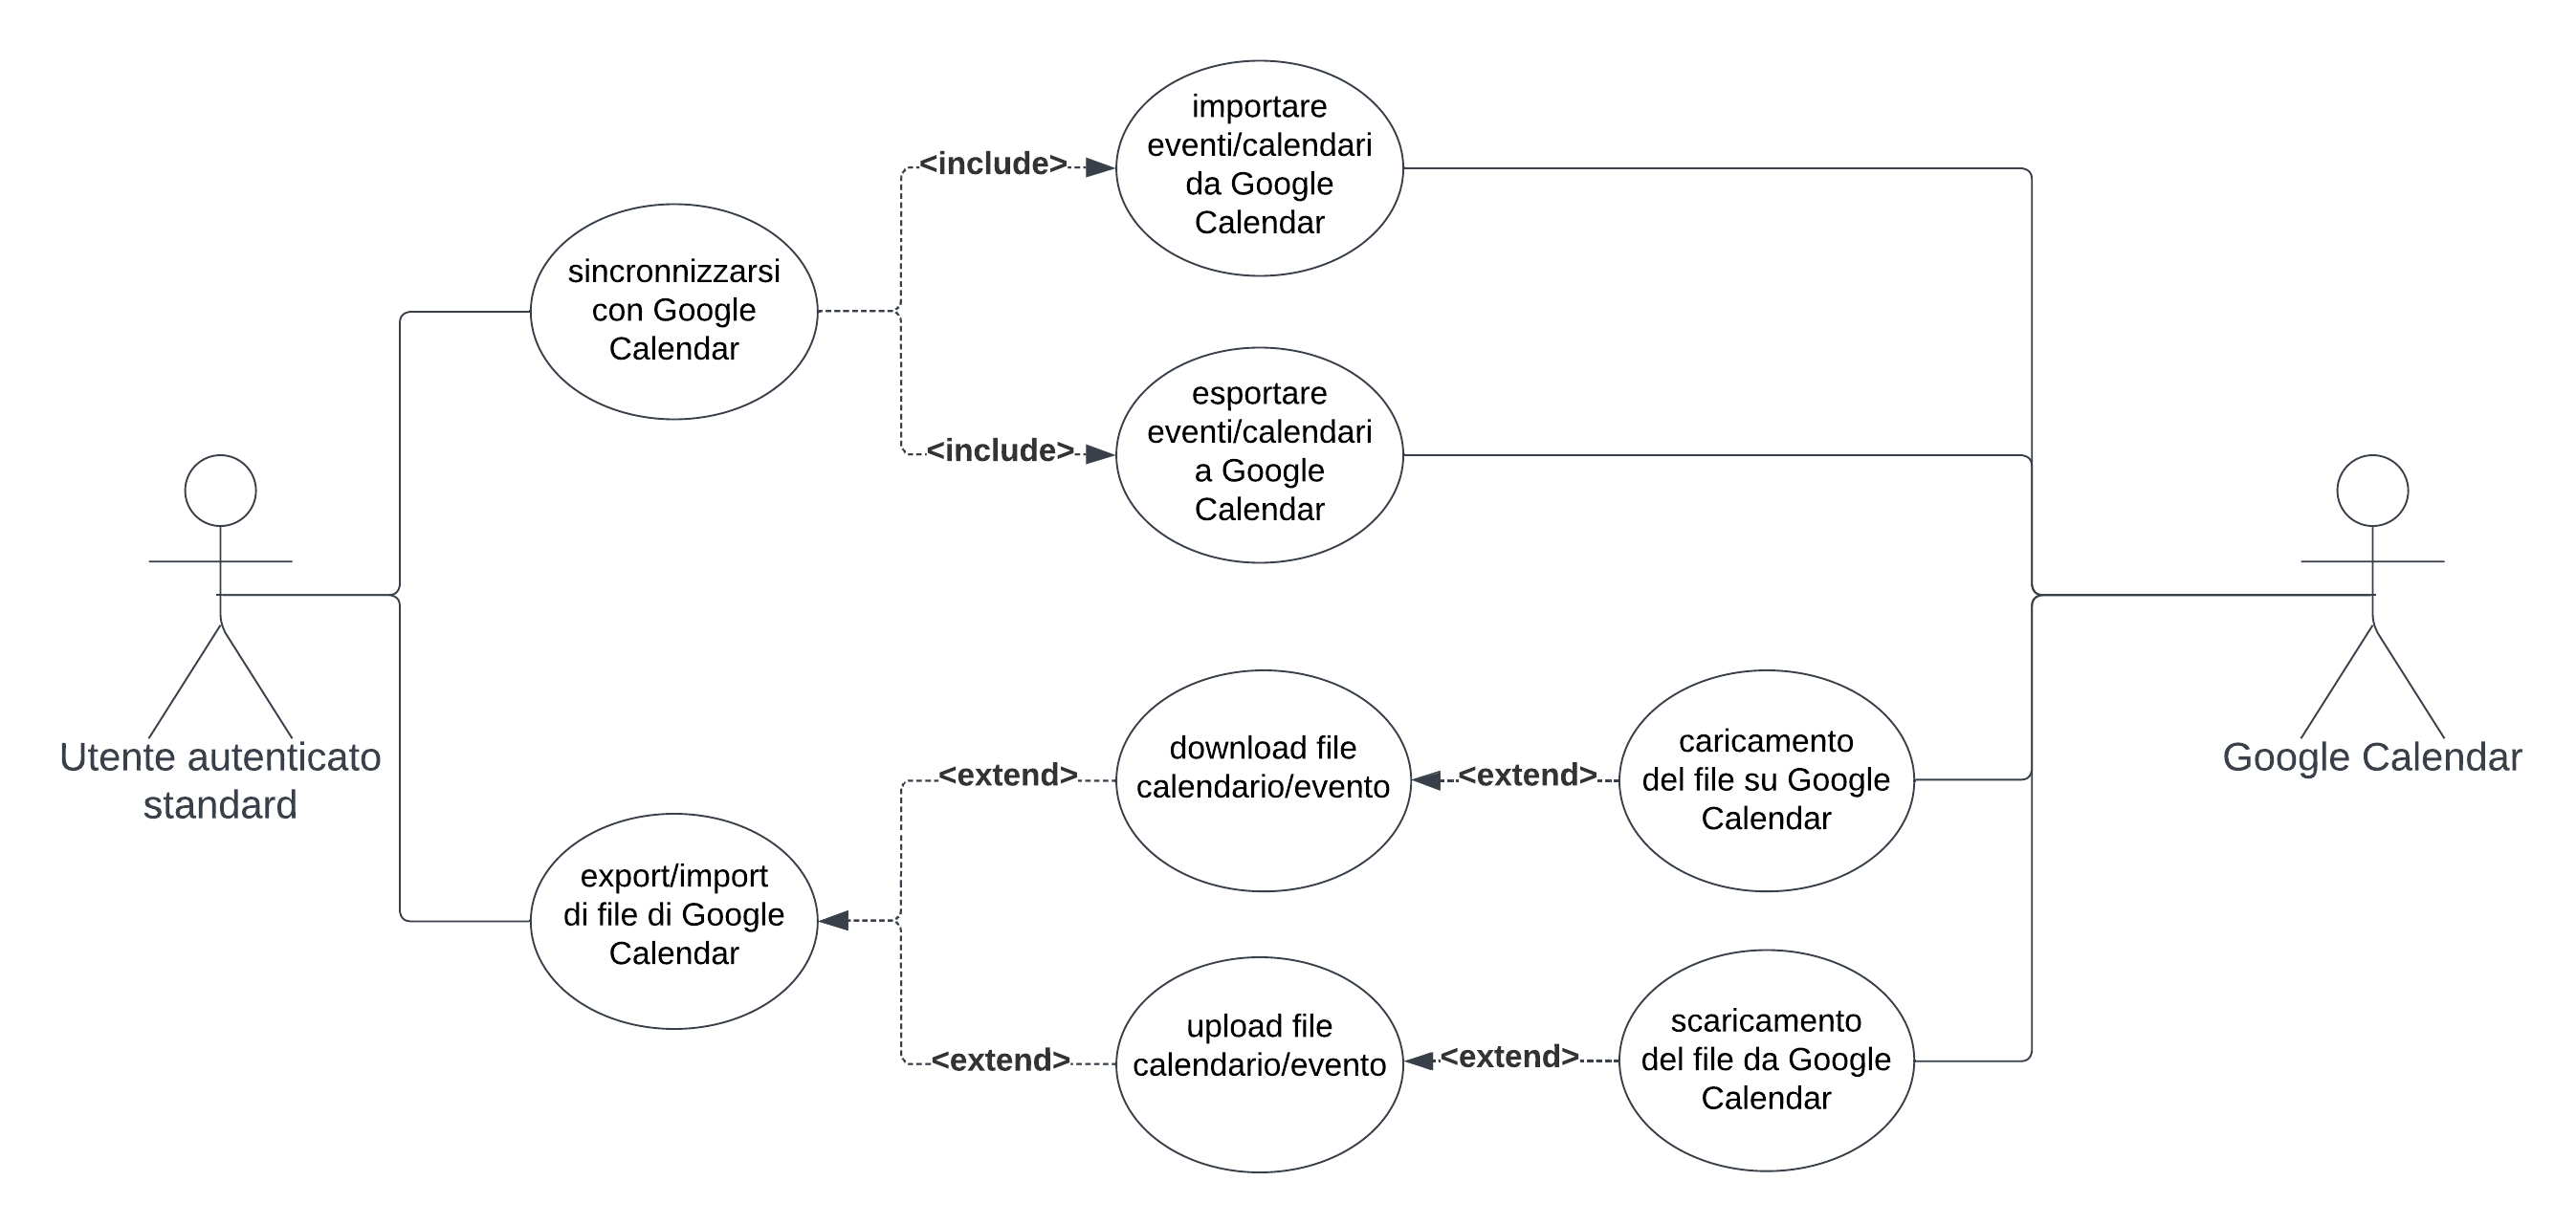
\includegraphics[width=0.8\textwidth]{img/Diagrammi/UseCases/GoogleCalendar.png}
        \end{center}


        \textbf{Titolo:} interagire con Google Calendar.

        \textbf{Riassunto:} \\
        Questo use case descrive come il sistema permetta all'utente autenticato standard l'utilizzo di Google Calendar tramite la piattaforma. Infatti, in quanto Google Calendar è un'applicazione molto diffusa, il sistema permette l'integrazione con questa applicazione. \\ 
        Questo use case è una specifica dell'use case "Impostazioni Account" in quanto la procedura di interazione con Google Calendar richiede una maggiore dettagliatezza e, per questo motivo, si è deciso di fare un use case a parte.
        

        \textbf{Descrizione:}
        \begin{enumerate}
            \item Da "Impostazioni Account" nella sezione "Interazione con Google Calendar" l'utente può andare ad interagire con Google Calendar. Premendo su "Interazione con Google Calendar" viene data la scelta all'utente o di sincronizzare il suo account di PlanIt con Google Calendar o di importare o esportare calendari o eventi via file.
            \item L'utente autenticato standard potrà decidere se connettere il proprio account Google Calendar al proprio account. Premendo su "Sincronizza con Google Calendar" inizia la procedura di connessione del proprio account di PlanIt con Google Calendar. Infatti tramite un'apposita finestra di dialogo, l'utente autenticato standard farà l'accesso al proprio account Google e concederà alla piattaforma i permessi per interagire con il calendario di Google Calendar \ref{uc:ExceptionInterruzioneSincronizzazione}. Una volta concessa l'autorizzazione si potrà scegliere quale calendario sincronizzare, se sincronizzare gli eventi da e/o verso Google Calendar.
            \item In alternativa nella sezione “importa/esporta” della piattaforma si potrà trovare un casella dove si può caricare un file di calendario o evento Google Calendar che si vuole importare \ref{uc:ExceptionErroreUpload} su PlanIt e un tasto, che premendolo fornisce il file di calendario \ref{uc:ExceptionErroreDownload} con cui si può esportare il proprio calendario di PlanIt su Google Calendar. \ref{uc:ExceptionFileNonValidoOCorrotto}.
        \end{enumerate}

        \textbf{Exceptions:}
        \begin{enumerate}[label=\textbf{[exception \arabic{enumiii}]}, ref= \textbf{[exception \arabic{enumiii}]}]
            \elemento{uc:ExceptionInterruzioneSincronizzazione} Nel caso in cui l'utente autenticato standard decidesse d'interrompere la procedura di autenticazione/gestione consensi l'attività d'importazione/esportazione non andrà a termine.
            \elemento{uc:ExceptionErroreUpload} Nel caso l'utente autenticato standard non finisse di caricare il file, il calendario da file caricato non potrà essere caricato sulla piattaforma in quanto mancherebbero informazioni.
            \elemento{uc:ExceptionErroreDownload} Se dopo aver richiesto alla piattaforma di esportare il proprio calendario su file si chiude la piattaforma prima d'iniziare il download del file, lo scaricamento del file non avverrà.
            \elemento{uc:ExceptionFileNonValidoOCorrotto} Nel caso il file caricato non sia valido oppure corrotto, verrà mostrato un messaggio di errore chiedendo di caricare un file diverso.
        \end{enumerate}

        \todo{Forse bisogna cambiare l'importazione esportazione automatica in sincronizzazione nel Diagramma, mi sembra tutto a posto.}
    \end{listaPersonale2}

    \newpage
    \elemento[Use case “Recupero password” (\prettyref{D1-rf:RecuperoPassword})]{uc:RecuperoPassword}

    \begin{center}
        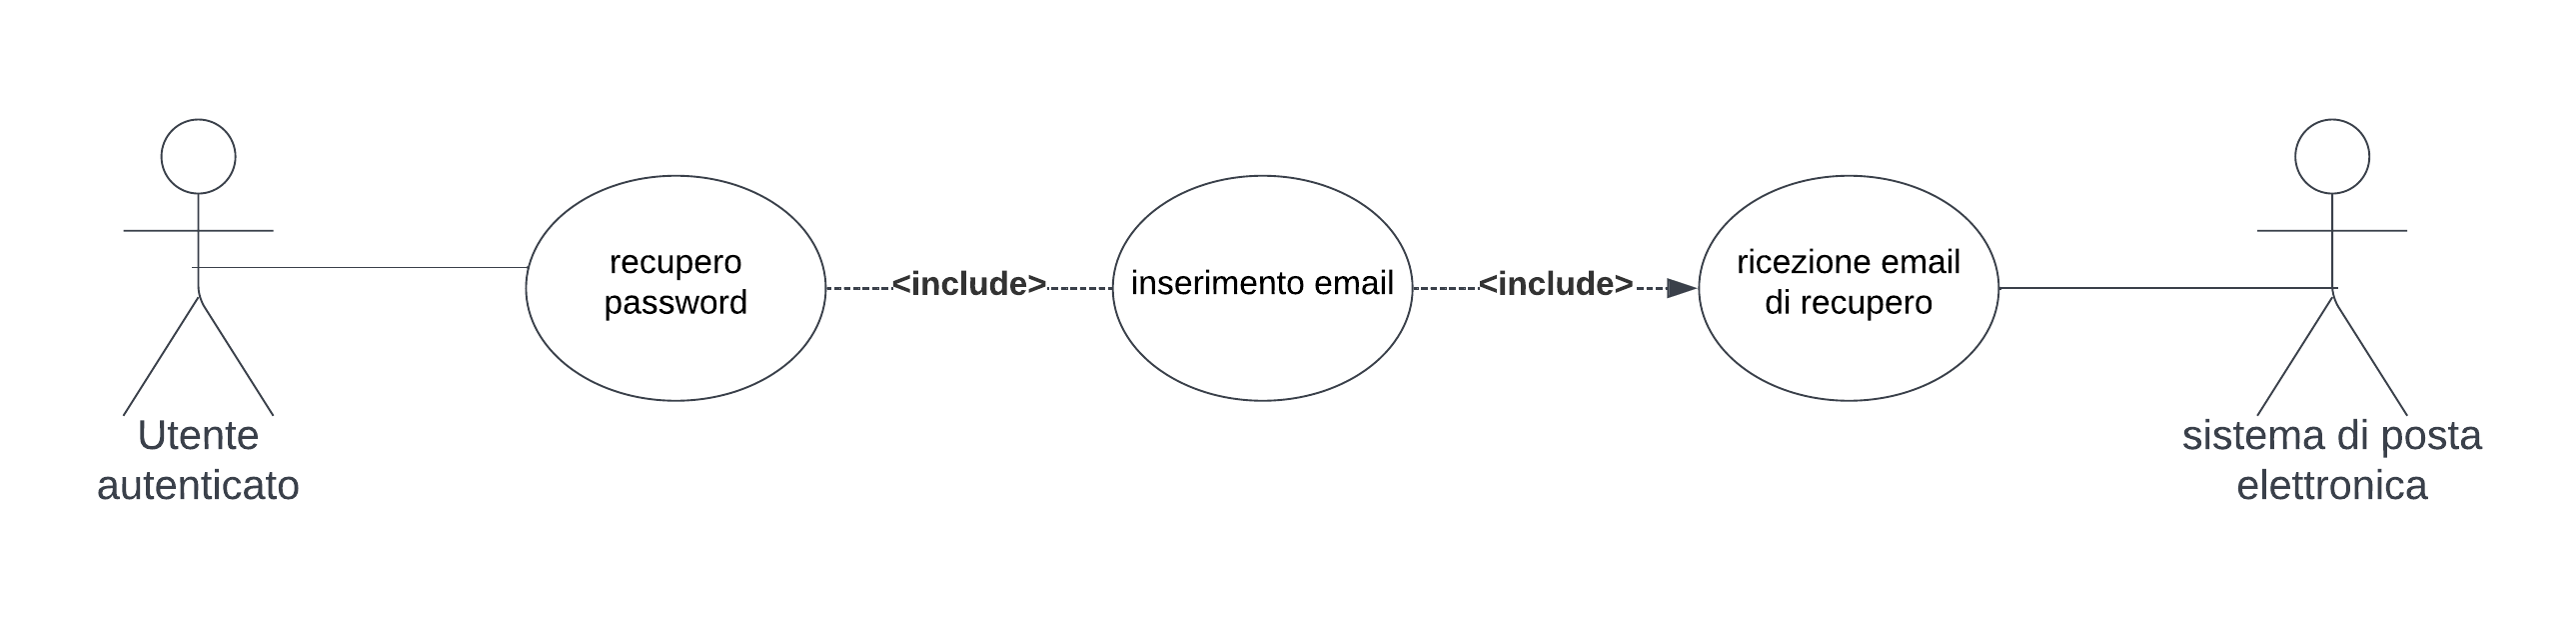
\includegraphics[width=0.7\textwidth]{img/Diagrammi/UseCases/RecuperoPassword.png}
    \end{center}
    Per descrivere questo use case, si è deciso di utilizzare un Sequence Diagram a discapito di una descrizione in italiano, per poter evidenziare meglio la procedura che deve essere effettuata per il recupero e reset della password.

    \textbf{Diagramma:}
    \begin{center}
        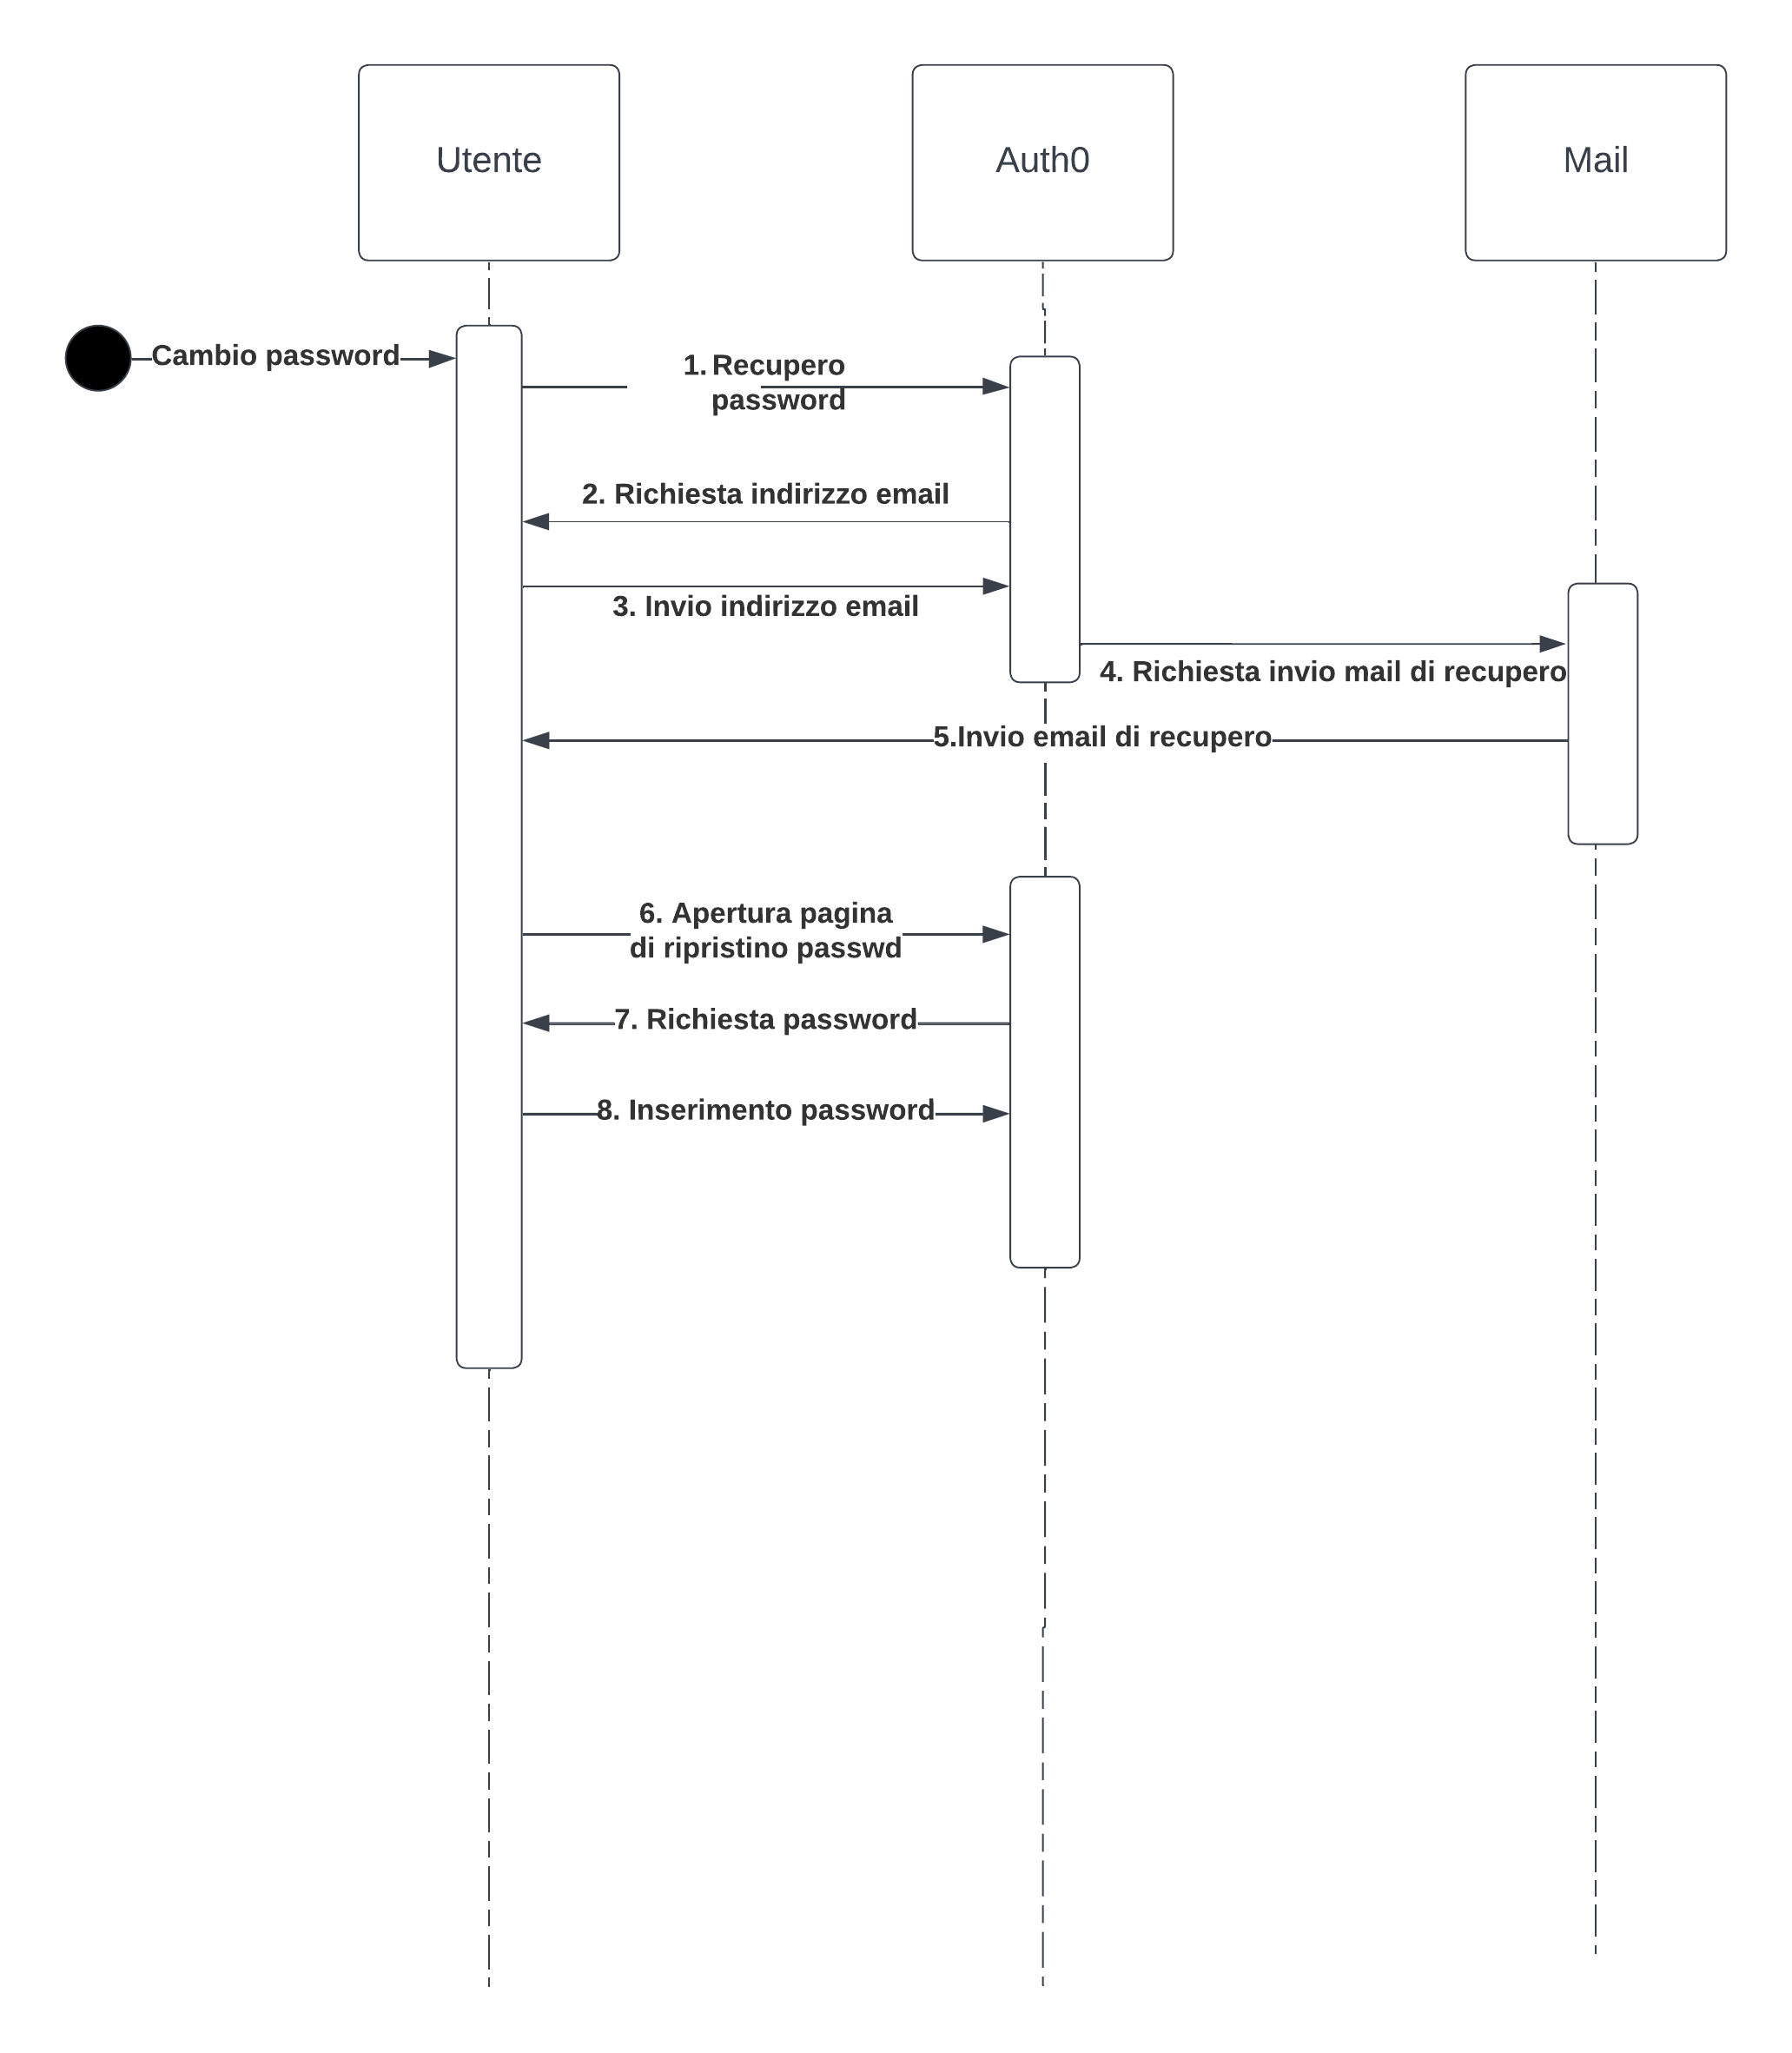
\includegraphics[width=0.7\textwidth]{img/Diagrammi/DS/DS_RecuperoPassword.png}
    \end{center}

\end{listaPersonale}